% Saberes básicos (LOMLOE) asociados a esta unidad
%
% B. La materia
%   - Teoría cinético-molecular: aplicación a observaciones sobre la materia explicando
%     sus propiedades, los estados de agregación y los cambios de estado. Es el eje
%     central de la unidad: toda la unidad explica los estados de agregación (sólido,
%     líquido, gas) y los cambios de estado (fusión, ebullición, evaporación,
%     sublimación...) a partir del modelo de partículas en movimiento.
%   - Experimentos relacionados con los sistemas materiales: conocimiento y descripción
%     de sus propiedades. Se describen propiedades como la compresibilidad, la
%     densidad relativa de los estados o la presión de un gas, ligadas al
%     comportamiento de las partículas.
%
% C. La energía
%   - Efectos del calor sobre la materia: análisis de los efectos y aplicación en
%     situaciones cotidianas. Se estudia cómo el calor produce cambios de estado, la
%     curva de calentamiento/enfriamiento y el concepto de calor latente, así como
%     fenómenos cotidianos (niebla, rocío, olla a presión, altitud y ebullición...).
%
% A. Las destrezas científicas básicas
%   - El lenguaje científico: unidades del Sistema Internacional. Se usan
%     sistemáticamente unidades de presión, volumen y temperatura (atmósferas, litros,
%     kelvin) y el manejo de \qty{}{} de siunitx en los ejemplos y ejercicios numéricos
%     de las leyes de los gases.
%   - Estrategias de interpretación y producción de información científica. Se
%     interpretan tablas de puntos de fusión/ebullición y gráficas de calentamiento
%     descritas verbalmente para extraer conclusiones.

\spacing{1.3}
\raggedbottom % pages with large figures end where the text ends (no stretched gaps between boxes)

\section{Estados físicos de la materia}

En la Tierra, casi todo lo que nos rodea es un \textbf{sólido}, un \textbf{líquido} o un \textbf{gas}. Cada estado tiene su propia «personalidad»:

\begin{figure}[H]
    \centering
    % [FIGURA ORIGINAL] \includegraphics[width=\textwidth]{Unit_2/states_overview}
    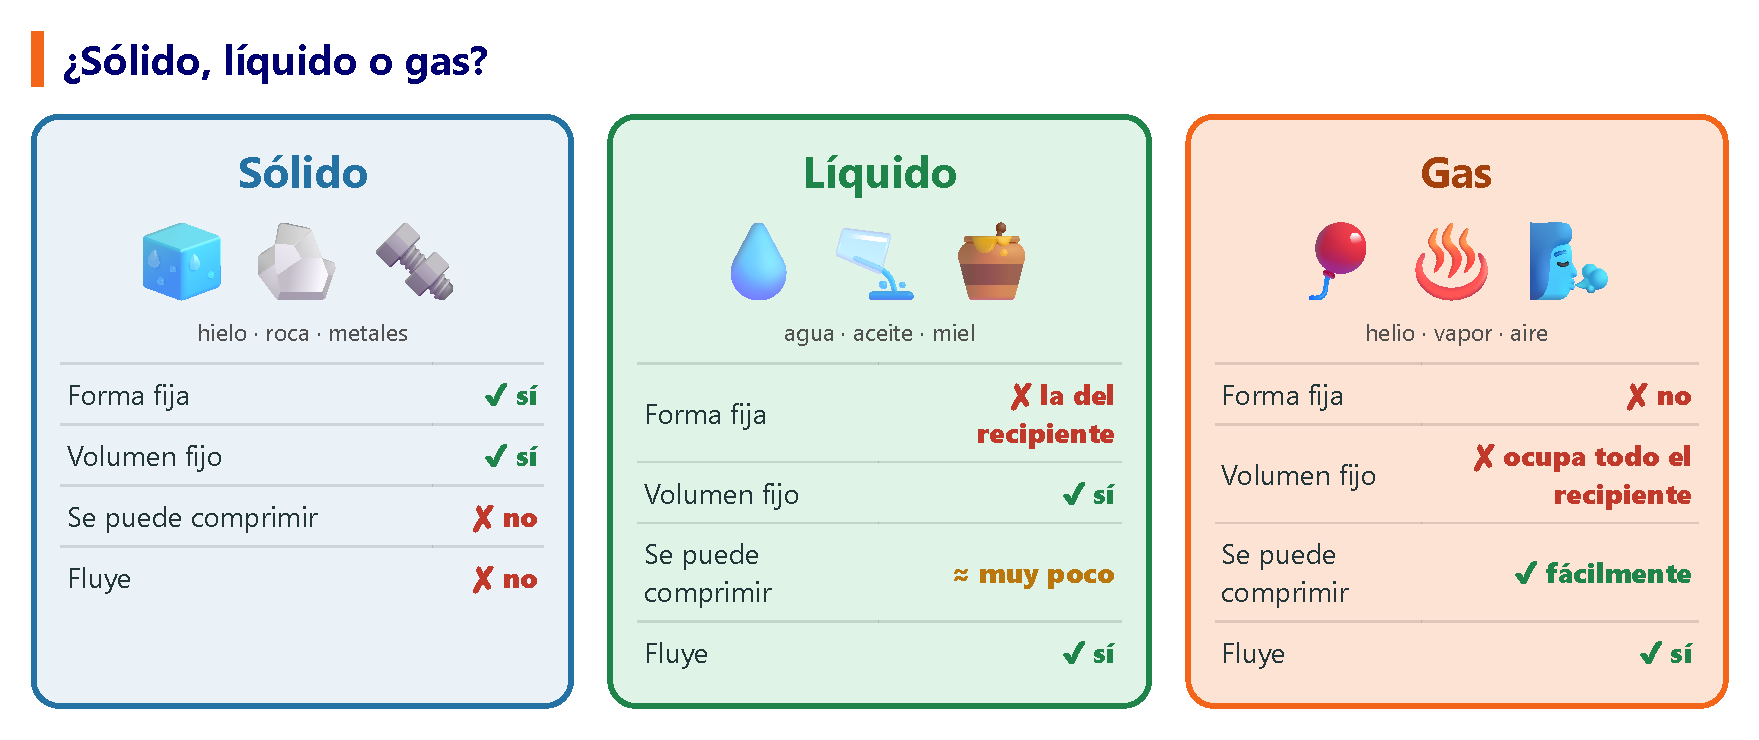
\includegraphics[width=\textwidth]{FigurasSVG/Unit_2_State_of_Matter/pdf/states_overview_es.pdf}
    \caption{Propiedades de los sólidos, los líquidos y los gases.}
    \label{fig:u2_states_overview}
\end{figure}

\subsection{El plasma: el cuarto estado de la materia}

Sólido, líquido y gas no son los únicos estados de la materia. Existe un \negsubro{cuarto estado}, llamado \textbf{plasma}.

\begin{definition}[Plasma]
    Un gas tan \textbf{caliente} que sus partículas se rompen y quedan \textbf{cargadas eléctricamente}. Por eso el plasma \textbf{brilla} (emite luz) y conduce la electricidad. Se considera el \textbf{cuarto estado de la materia}.
\end{definition}

\begin{figure}[H]
    \centering
    % [FIGURA ORIGINAL] \includegraphics[width=\textwidth]{Unit_2/plasma}
    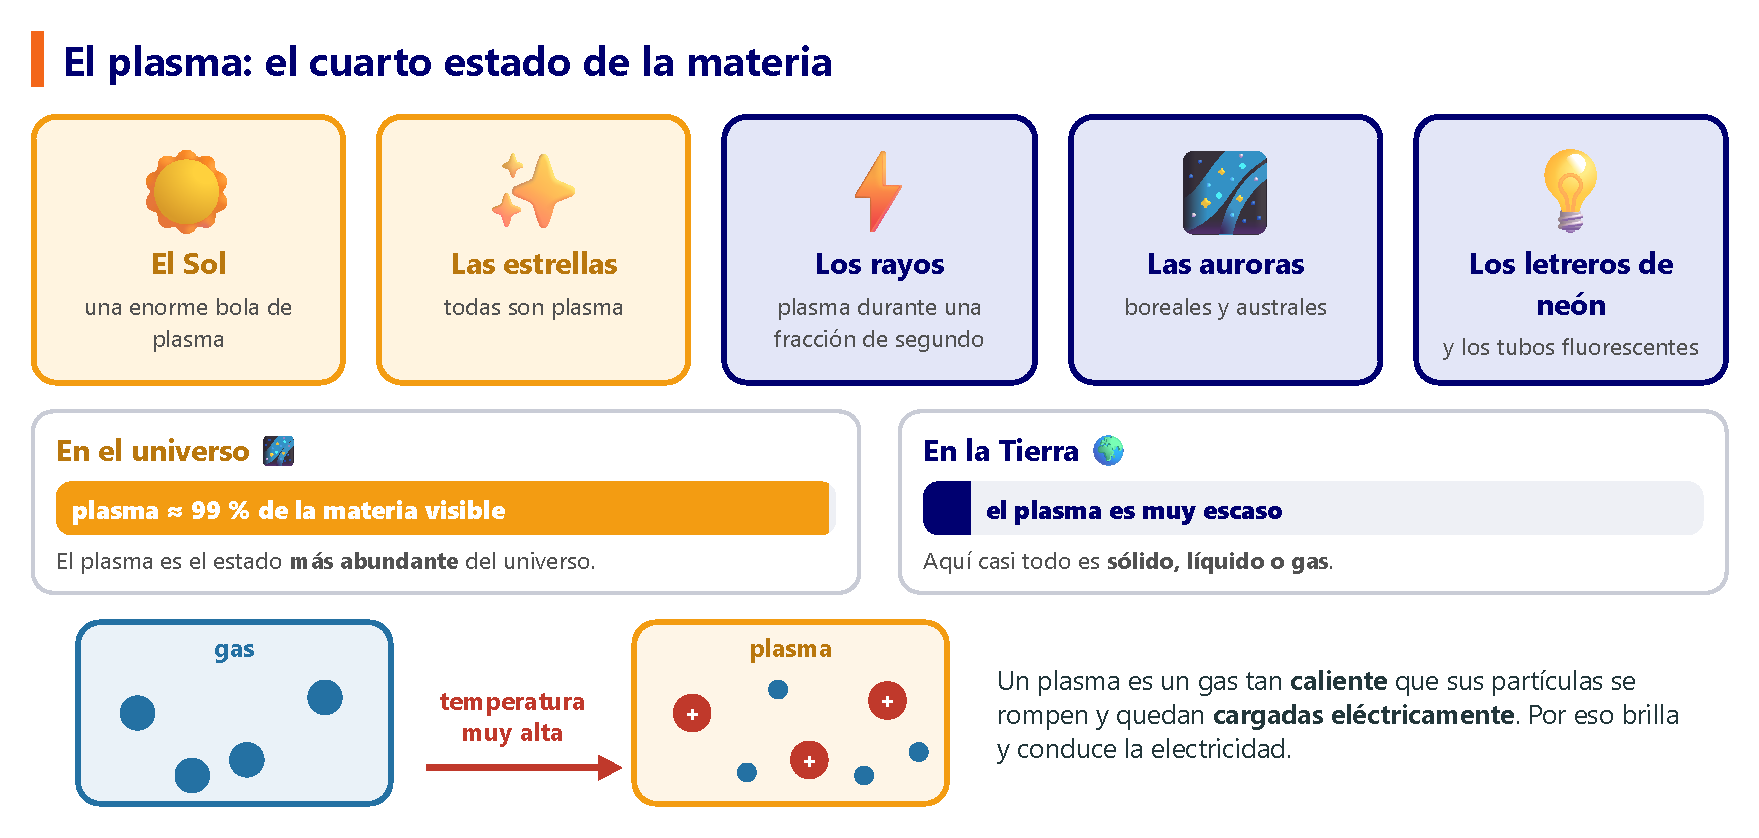
\includegraphics[width=\textwidth]{FigurasSVG/Unit_2_State_of_Matter/pdf/plasma_es.pdf}
    \caption{El plasma es el estado más abundante del universo, pero en la Tierra es muy escaso.}
    \label{fig:u2_plasma}
\end{figure}

\begin{impt}
    \begin{itemize}
        \item El plasma es el estado de la materia \textbf{más abundante del universo}: el \textbf{Sol} y todas las estrellas son enormes bolas de plasma.
        \item En la \textbf{Tierra}, en cambio, el plasma es \textbf{muy escaso}: solo lo vemos en los rayos, en las auroras (auroras boreales) y en los letreros de neón y los tubos fluorescentes.
    \end{itemize}
\end{impt}

\begin{didyouknow}
    También existen los \textbf{cristales líquidos}, un estado curioso a medio camino entre líquido y sólido. Se usan en las pantallas LCD de los móviles y los televisores.
\end{didyouknow}

\begin{exercise}
    Clasifica cada sustancia como sólido, líquido o gas a temperatura ambiente: madera, gas natural, aceite, agua, aluminio, oxígeno, alcohol, dióxido de carbono, arena.
    \begin{solu}
        \textbf{Sólidos}: madera, aluminio, arena. \\
        \textbf{Líquidos}: aceite, agua, alcohol. \\
        \textbf{Gases}: gas natural, oxígeno, dióxido de carbono.
    \end{solu}
\end{exercise}

\begin{exercise}
    Responde a estas preguntas sobre el plasma:
    \begin{enumerate}[label=\letraminuscula]
        \item ¿Por qué se llama al plasma el «cuarto estado de la materia»?
        \item ¿Cuál es el estado de la materia más abundante en el universo? ¿Y en la Tierra?
        \item Pon dos ejemplos de plasma que puedas ver en la Tierra.
    \end{enumerate}
    \begin{solu}
        \begin{enumerate}[label=\alph*)]
            \item Porque es distinto de los sólidos, los líquidos y los gases: es un gas tan caliente que sus partículas tienen carga eléctrica.
            \item En el universo, el plasma (el Sol y las estrellas). En la Tierra el plasma es muy escaso: la mayor parte de la materia es sólida, líquida o gaseosa.
            \item Los rayos, las auroras, los letreros de neón, los tubos fluorescentes.
        \end{enumerate}
    \end{solu}
\end{exercise}

\begin{exercise}
    Indica si cada afirmación es verdadera o falsa, y corrige las falsas.
    \begin{enumerate}[label=\letraminuscula]
        \item La arena fluye, así que es un líquido.
        \item Una esponja se puede comprimir, así que es un gas.
        \item La esponja está hecha de un material poroso y flexible con aire en su interior, por eso se puede comprimir.
    \end{enumerate}
    \begin{solu}
        \begin{enumerate}[label=\alph*)]
            \item \textbf{Falsa}. La arena es un sólido formado por granos muy pequeños que parecen comportarse como un líquido, pero cada grano conserva su forma y su tamaño.
            \item \textbf{Falsa}. Una esponja es un sólido; se puede comprimir porque es porosa (tiene aire dentro), no porque sea un gas.
            \item \textbf{Verdadera}.
        \end{enumerate}
    \end{solu}
\end{exercise}

\begin{exercise}
    Una alumna tiene tres jeringuillas cerradas iguales: la jeringuilla A contiene aire, la B contiene agua y la C contiene una pequeña bola de metal. Tapa la punta de cada jeringuilla y empuja el émbolo con toda su fuerza.
    \begin{enumerate}[label=\letraminuscula]
        \item ¿En qué jeringuilla se puede hundir claramente el émbolo?
        \item Explica el resultado a partir de la compresibilidad de los sólidos, los líquidos y los gases.
    \end{enumerate}
    \begin{solu}
        \begin{enumerate}[label=\alph*)]
            \item Solo en la \textbf{jeringuilla A} (la que tiene aire).
            \item Los gases se pueden comprimir porque hay mucho espacio vacío entre sus partículas. Los líquidos (jeringuilla B) y los sólidos (jeringuilla C) no se pueden comprimir, ya que sus partículas casi se tocan.
        \end{enumerate}
    \end{solu}
\end{exercise}

%----------------------------------------------------------------------------------------

\section{Teoría cinética y estados de la materia}

¿Por qué el hielo es duro, el agua fluye y el vapor es invisible, si los tres son la misma sustancia? Para responder a esta pregunta, los científicos imaginan la materia como si estuviera formada por «bolitas» diminutas. Esta idea se llama \negsubro{teoría cinética} («cinética» viene de una palabra griega que significa «movimiento»).

\begin{definition}[Teoría cinética]
    Modelo científico que explica cómo se comporta la materia imaginando que está formada por \textbf{partículas} diminutas que están \textbf{siempre en movimiento}.
\end{definition}

La teoría cinética se puede resumir en cuatro ideas sencillas:

\begin{enumerate}[label=\numberballmDarkTeal]
    \item \textbf{Todo está formado por partículas.} Toda la materia está formada por partículas tan pequeñas que no podemos verlas, ni siquiera con un microscopio normal.
    \item \textbf{Las partículas nunca dejan de moverse.} Vibran, se desplazan y chocan entre sí continuamente.
    \item \textbf{Más caliente significa más rápido.} Cuando calentamos una sustancia, sus partículas se mueven más deprisa; cuando la enfriamos, se mueven más despacio. La \textbf{temperatura} nos dice lo rápido que se mueven las partículas.
    \item \textbf{Las partículas se atraen entre sí.} Están unidas por fuerzas, como si hubiera un «pegamento» invisible. Lo fuerte que sea ese pegamento, comparado con lo rápido que se mueven las partículas, decide si la sustancia es un \textbf{sólido}, un \textbf{líquido} o un \textbf{gas}.
\end{enumerate}

\begin{impt}
    Piensa en el alumnado de tu instituto: en clase cada uno está sentado en su sitio y solo se mueve un poco (\textbf{sólido}); en el pasillo caminan y se cruzan unos con otros, pero siguen muy juntos (\textbf{líquido}); en el patio corren libremente en todas direcciones, lejos unos de otros (\textbf{gas}).
\end{impt}

\begin{figure}[H]
    \centering
    % [FIGURA ORIGINAL] \includegraphics[width=\textwidth]{Unit_2/particle_model}
    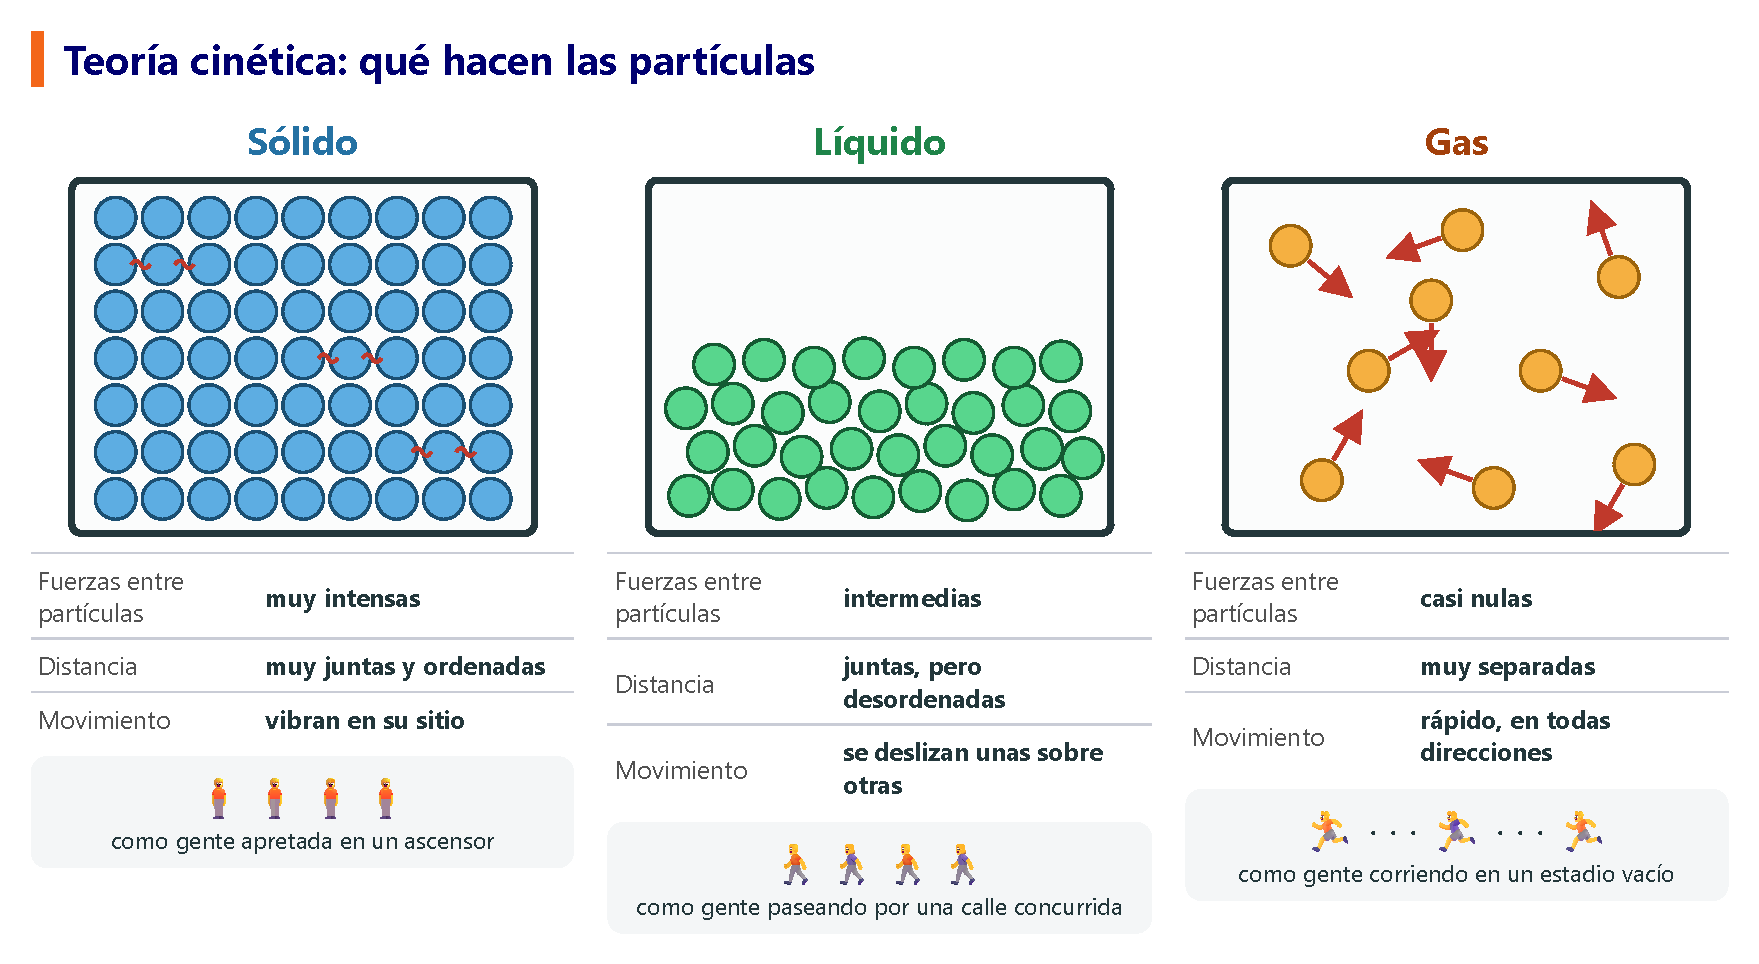
\includegraphics[width=\textwidth]{FigurasSVG/Unit_2_State_of_Matter/pdf/particle_model_es.pdf}
    \caption{Modelo de partículas de los tres estados de la materia.}
    \label{fig:u2_particle_model}
\end{figure}

\begin{impt}
    Como sus partículas están tan juntas, los sólidos suelen tener la densidad \textbf{más alta}, los líquidos algo menor y los gases una densidad \textbf{muy baja}.
\end{impt}

\subsection{La presión de un gas}

\begin{definition}[Presión de un gas]
    Es el resultado de los \textbf{choques} de las partículas de un gas \textbf{contra las paredes} del recipiente. Más choques, o choques más fuertes, suponen más presión.
\end{definition}

\begin{figure}[H]
    \centering
    % [FIGURA ORIGINAL] \includegraphics[width=\textwidth]{Unit_2/gas_pressure}
    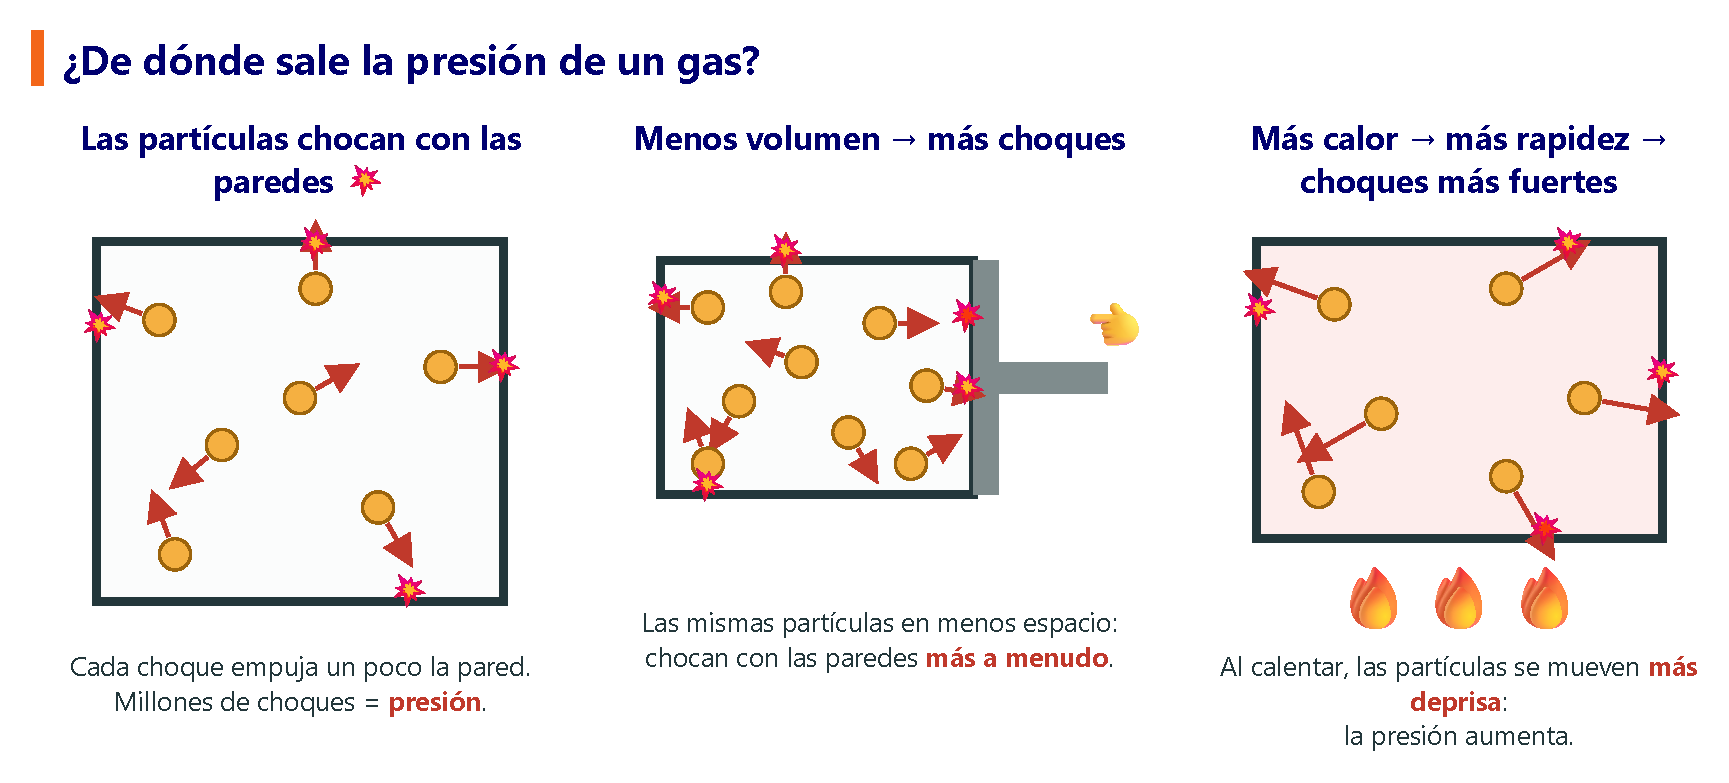
\includegraphics[width=\textwidth]{FigurasSVG/Unit_2_State_of_Matter/pdf/gas_pressure_es.pdf}
    \caption{La presión de un gas aumenta si disminuye el volumen o si aumenta la temperatura.}
    \label{fig:u2_gas_pressure}
\end{figure}

\begin{exercise}
    Utiliza la teoría cinética para explicar por qué un bloque de metal se dilata un poco cuando se calienta, pero no cambia de estado.
    \begin{solu}
        Al calentarlo, las partículas del sólido vibran más, así que la distancia entre ellas aumenta ligeramente; pero las fuerzas entre las partículas siguen siendo lo bastante fuertes para mantener la estructura rígida, de modo que la sustancia sigue siendo un sólido, solo que un poco más grande.
    \end{solu}
\end{exercise}

\begin{exercise}
    Un iceberg flota en el mar.
    \begin{enumerate}[label=\letraminuscula]
        \item Utiliza la teoría cinética para explicar si las partículas están más separadas en el hielo o en el agua líquida.
        \item ¿Qué le pasará al nivel del mar si el iceberg se derrite?
    \end{enumerate}
    \begin{solu}
        \begin{enumerate}[label=\alph*)]
            \item Como el hielo flota, es \textbf{menos denso} que el agua líquida; por tanto, sus partículas están \textbf{más separadas} en el sólido que en el líquido (en esto el agua es una sustancia poco habitual).
            \item El iceberg ya está flotando, así que ya desplaza un volumen de agua equivalente a su propio peso; cuando se derrite, el nivel del mar \textbf{no} sube (al contrario que el hielo que se funde sobre tierra firme, que añade agua nueva al mar).
        \end{enumerate}
    \end{solu}
\end{exercise}

\begin{exercise}
    La densidad de algunos gases a temperatura ambiente es: oxígeno \qty{1.33}{\kg\per\cubic\metre}, helio \qty{0.17}{\kg\per\cubic\metre}, aire \qty{1.20}{\kg\per\cubic\metre}. Explica por qué los globos de helio suben en el aire, mientras que unos globos de oxígeno no lo harían.
    \begin{solu}
        Un globo sube en el aire cuando es \textbf{menos denso} que el aire. El helio (\qty{0.17}{\kg\per\cubic\metre}) es mucho menos denso que el aire (\qty{1.20}{\kg\per\cubic\metre}), así que sube. El oxígeno (\qty{1.33}{\kg\per\cubic\metre}) es más denso que el aire, así que un globo de oxígeno caería.
    \end{solu}
\end{exercise}

\begin{exercise}
    Dos globos cerrados iguales se llenan con la misma cantidad de aire. Uno se deja en la nevera y el otro junto a un radiador. Utiliza la teoría cinética para predecir cuál de los dos acabará siendo más grande.
    \begin{solu}
        El globo que está junto al \textbf{radiador}. El calor hace que las partículas de aire de su interior se muevan más deprisa, así que chocan contra las paredes con más fuerza y más a menudo; la presión aumenta y empuja las paredes hacia fuera. En el globo frío las partículas se mueven más despacio, la presión es menor y el globo se queda más pequeño.
    \end{solu}
\end{exercise}

\subsection{La teoría cinética explica fenómenos cotidianos}

\begin{figure}[H]
    \centering
    % [FIGURA ORIGINAL] \includegraphics[width=\textwidth]{Unit_2/everyday_kinetic}
    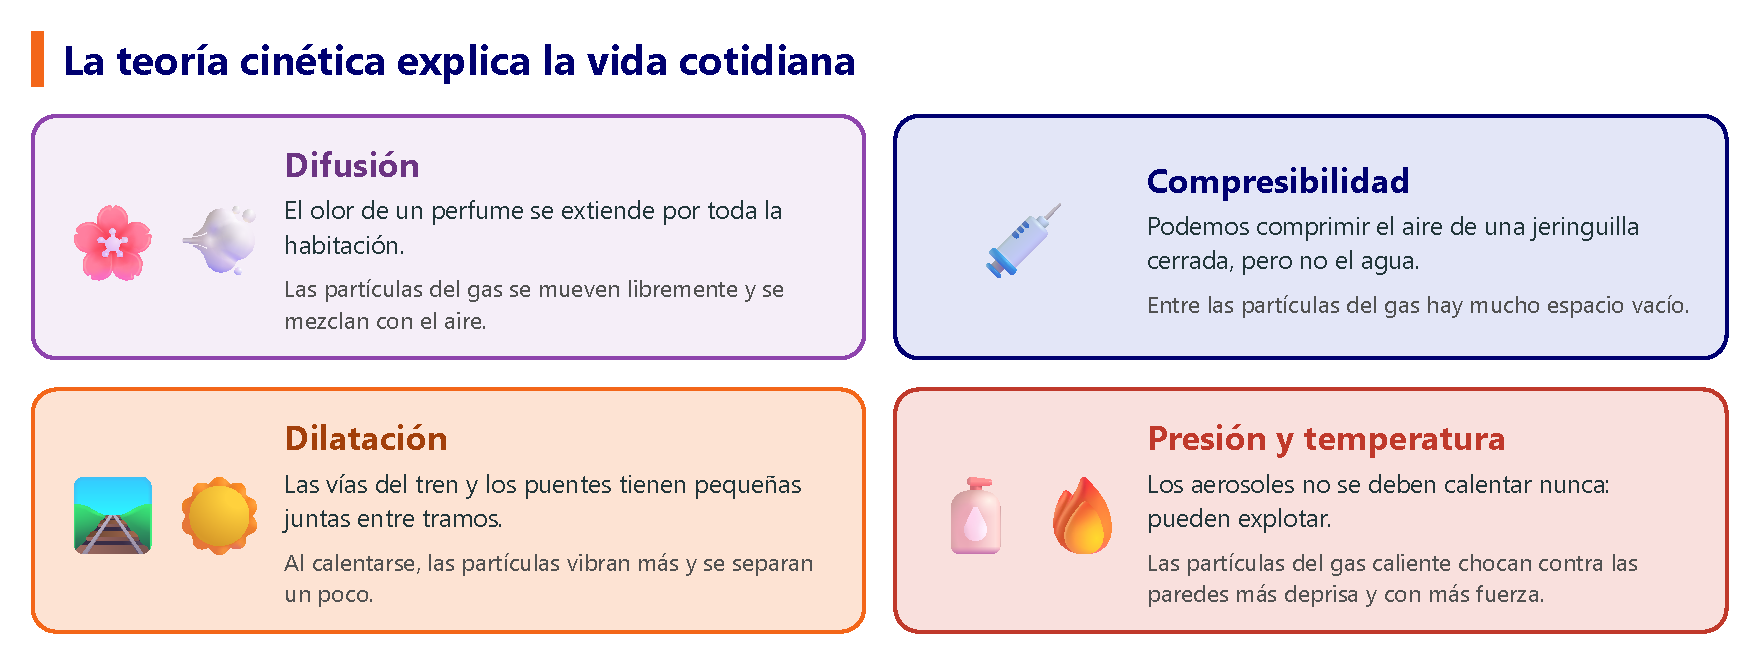
\includegraphics[width=\textwidth]{FigurasSVG/Unit_2_State_of_Matter/pdf/everyday_kinetic_es.pdf}
    \caption{Cuatro fenómenos cotidianos explicados con partículas.}
    \label{fig:u2_everyday_kinetic}
\end{figure}

\begin{definition}[Difusión]
    Proceso por el que las partículas de una sustancia se van extendiendo hasta mezclarse por completo con las partículas de otra. Es rápida en los gases y más lenta en los líquidos (una gota de tinta en agua).
\end{definition}

\begin{exercise}
    Utiliza la teoría cinética (difusión, dilatación, compresibilidad) para explicar cada situación.
    \begin{enumerate}[label=\letraminuscula]
        \item Desde otra habitación se huele la comida que se está cocinando en la cocina.
        \item La tapa metálica de un tarro de cristal se desenrosca con más facilidad después de ponerla bajo el chorro de agua caliente.
        \item Cuesta cada vez más empujar una bomba de bicicleta a medida que se comprime el aire de su interior.
    \end{enumerate}
    \begin{solu}
        \begin{enumerate}[label=\alph*)]
            \item Las partículas que desprende la comida se extienden por el aire por \textbf{difusión} hasta llegar a tu nariz.
            \item El calor hace que las partículas del metal de la tapa vibren más y se separen un poco, así que la tapa se \textbf{dilata} más que el cristal y queda más floja.
            \item El mismo número de partículas de gas se aprieta en un volumen más pequeño; chocan contra el émbolo más a menudo, así que la \textbf{presión} (y la fuerza necesaria para empujar) aumenta.
        \end{enumerate}
    \end{solu}
\end{exercise}

\begin{exercise}
    El perfume se extiende por una habitación más rápido en un día caluroso que en un día frío. Utiliza la teoría cinética para explicar por qué.
    \begin{solu}
        En un día caluroso las partículas se mueven, de media, \textbf{más deprisa} que en un día frío. La difusión se debe al movimiento desordenado de las partículas, así que, si son más rápidas, se extienden y se mezclan con el aire antes.
    \end{solu}
\end{exercise}

\begin{exercise}
    Una bolsa cerrada de patatas fritas tiene un aspecto normal al nivel del mar, pero cuando un avión sube a su altitud de crucero, la misma bolsa aparece hinchada.
    \begin{enumerate}[label=\letraminuscula]
        \item ¿Qué le ocurre a la presión del aire fuera de la bolsa a medida que el avión sube?
        \item Utiliza la teoría cinética para explicar por qué se hincha la bolsa.
    \end{enumerate}
    \begin{solu}
        \begin{enumerate}[label=\alph*)]
            \item La presión del aire \textbf{fuera} de la bolsa disminuye al aumentar la altitud.
            \item El aire de dentro de la bolsa sigue chocando contra las paredes interiores con la misma fuerza que antes, mientras que el aire de fuera empuja con menos fuerza. El empuje hacia fuera es mayor, así que la bolsa se hincha hasta que las presiones se igualan (o incluso puede reventar).
        \end{enumerate}
    \end{solu}
\end{exercise}

%----------------------------------------------------------------------------------------

\section{Leyes de los gases}

El comportamiento de un gas depende de tres magnitudes: la \textbf{presión} \(p\), el \textbf{volumen} \(V\) y la \textbf{temperatura} \(T\). Cada ley de los gases mantiene \textbf{una} de ellas constante y nos dice cómo se relacionan las otras dos.

\subsection{La escala Kelvin}

\begin{figure}[H]
    \centering
    % [FIGURA ORIGINAL] \includegraphics[width=0.95\textwidth]{Unit_2/kelvin_scale}
    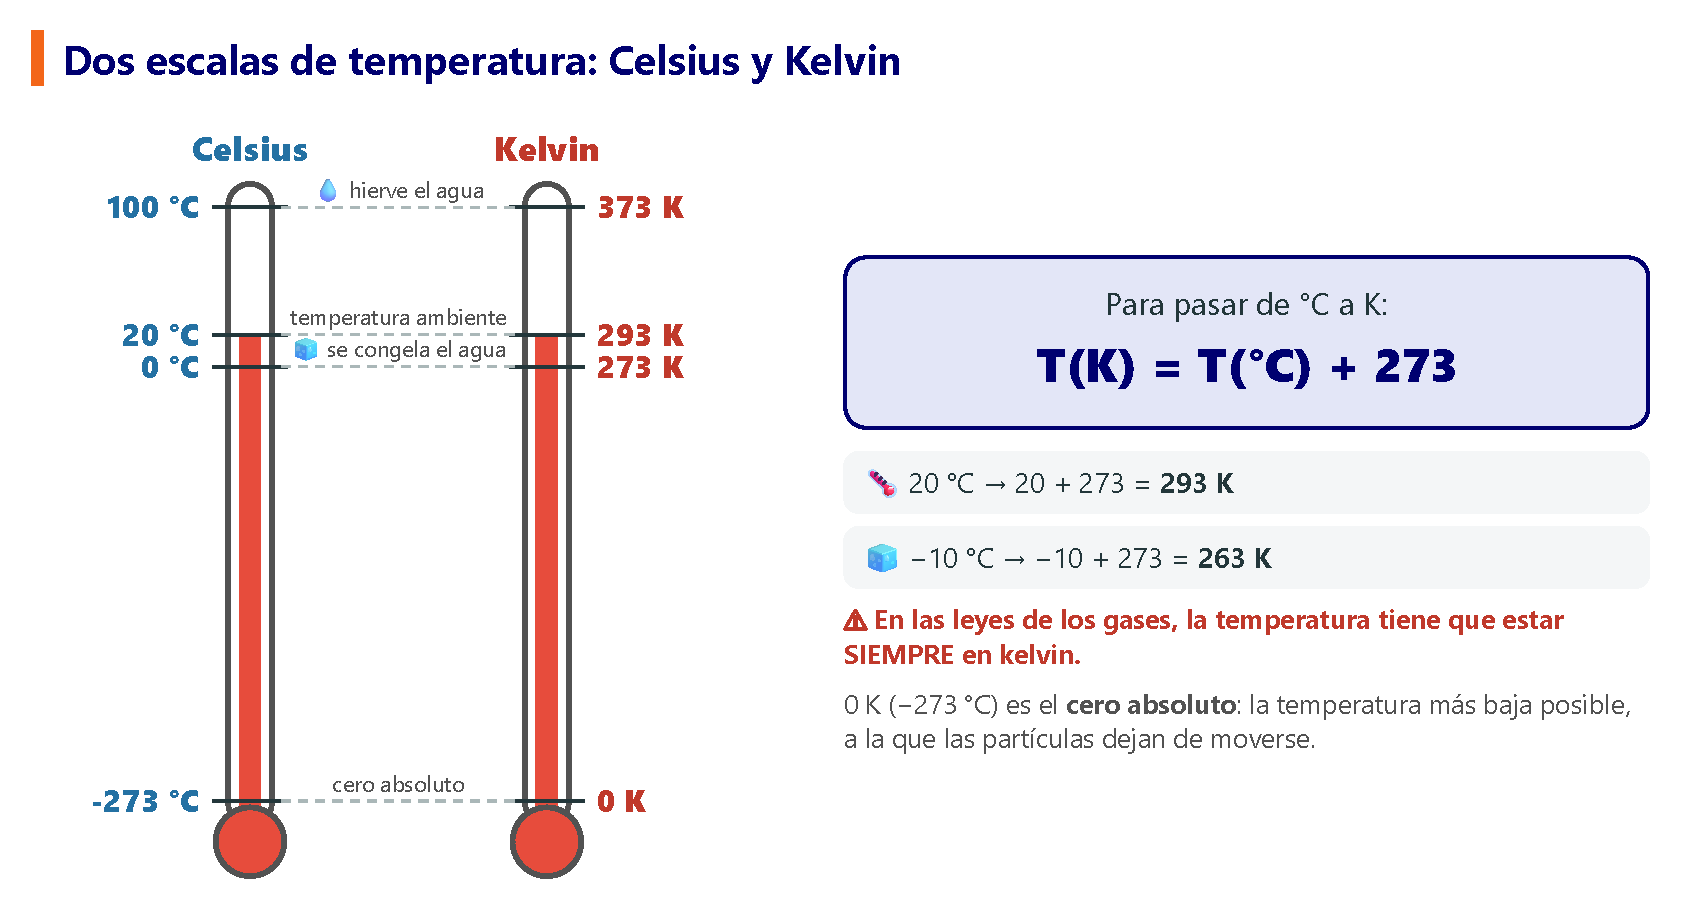
\includegraphics[width=0.95\textwidth]{FigurasSVG/Unit_2_State_of_Matter/pdf/kelvin_scale_es.pdf}
    \caption{Las escalas Celsius y Kelvin: el grado tiene el mismo tamaño, pero el cero está en otro sitio.}
    \label{fig:u2_kelvin_scale}
\end{figure}

\begin{impt}
    En \textbf{todas} las leyes de los gases, la temperatura tiene que estar en \textbf{kelvin}:
    \begin{equation*}
        T(\unit{\K}) = T(\unit{\celsius}) + 273
    \end{equation*}
\end{impt}

\subsection{¿Qué significan los números 1 y 2?}

En todas las leyes de los gases verás las magnitudes escritas con un numerito: \(p_1\), \(V_1\), \(T_1\) y \(p_2\), \(V_2\), \(T_2\). Estos numeritos se llaman \textbf{subíndices}, y son muy importantes:

\begin{impt}
    En las leyes de los gases siempre estudiamos el \textbf{mismo gas} en dos momentos distintos:
    \begin{itemize}
        \item El subíndice \textbf{1} indica el \textbf{principio} (el estado \textbf{inicial}): cómo está el gas \textbf{antes} del cambio.
        \item El subíndice \textbf{2} indica el \textbf{final} (el estado \textbf{final}): cómo está el gas \textbf{después} de que algo haya cambiado (lo calentamos, lo enfriamos, lo comprimimos o lo dejamos expandirse).
    \end{itemize}
    Por ejemplo, \(V_1\) es el volumen \textbf{antes} del cambio y \(V_2\) es el volumen \textbf{después} del cambio.
\end{impt}

\begin{figure}[H]
    \centering
    % [FIGURA ORIGINAL] \includegraphics[width=\textwidth]{Unit_2/states_1_2}
    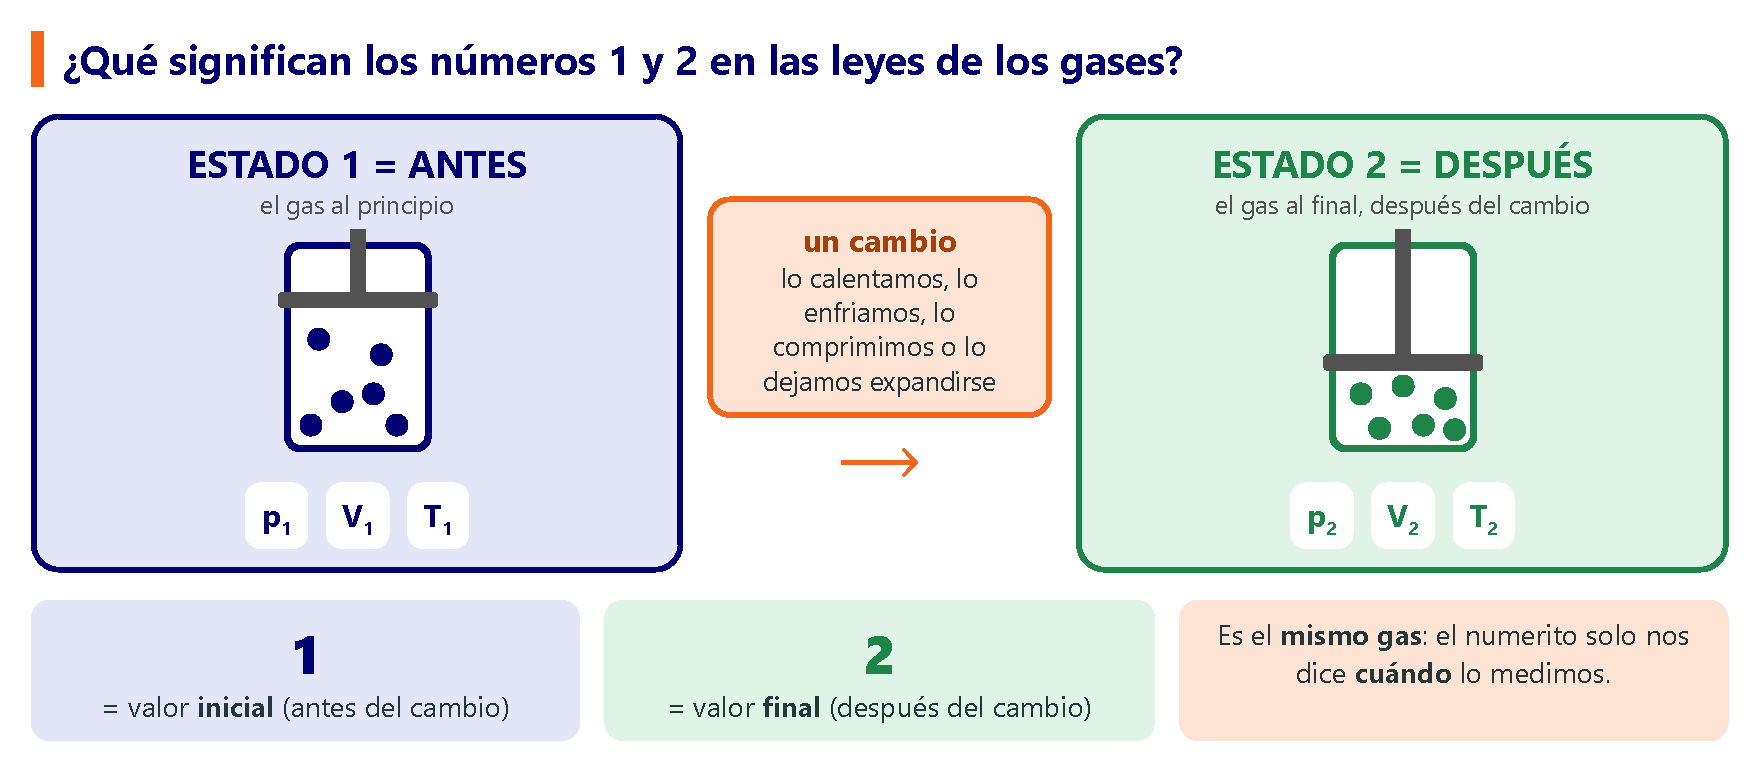
\includegraphics[width=\textwidth]{FigurasSVG/Unit_2_State_of_Matter/pdf/states_1_2_es.pdf}
    \caption{El estado 1 es el gas antes del cambio; el estado 2 es el mismo gas después del cambio.}
    \label{fig:u2_states_1_2}
\end{figure}

\begin{example}
    \textbf{«Un globo tiene un volumen de \qty{2}{\litre} a \qty{20}{\celsius}. Lo ponemos al sol y llega a \qty{40}{\celsius}.»} \\
    El \textbf{principio} es el globo antes de ponerlo al sol: \(V_1 = \qty{2}{\litre}\), \(T_1 = \qty{20}{\celsius}\). \\
    El \textbf{final} es el globo después de estar al sol: \(T_2 = \qty{40}{\celsius}\), y \(V_2\) es lo que tendríamos que calcular.
\end{example}

\subsection{Las tres leyes de los gases}

\begin{figure}[H]
    \centering
    % [FIGURA ORIGINAL] \includegraphics[width=\textwidth]{Unit_2/gas_laws}
    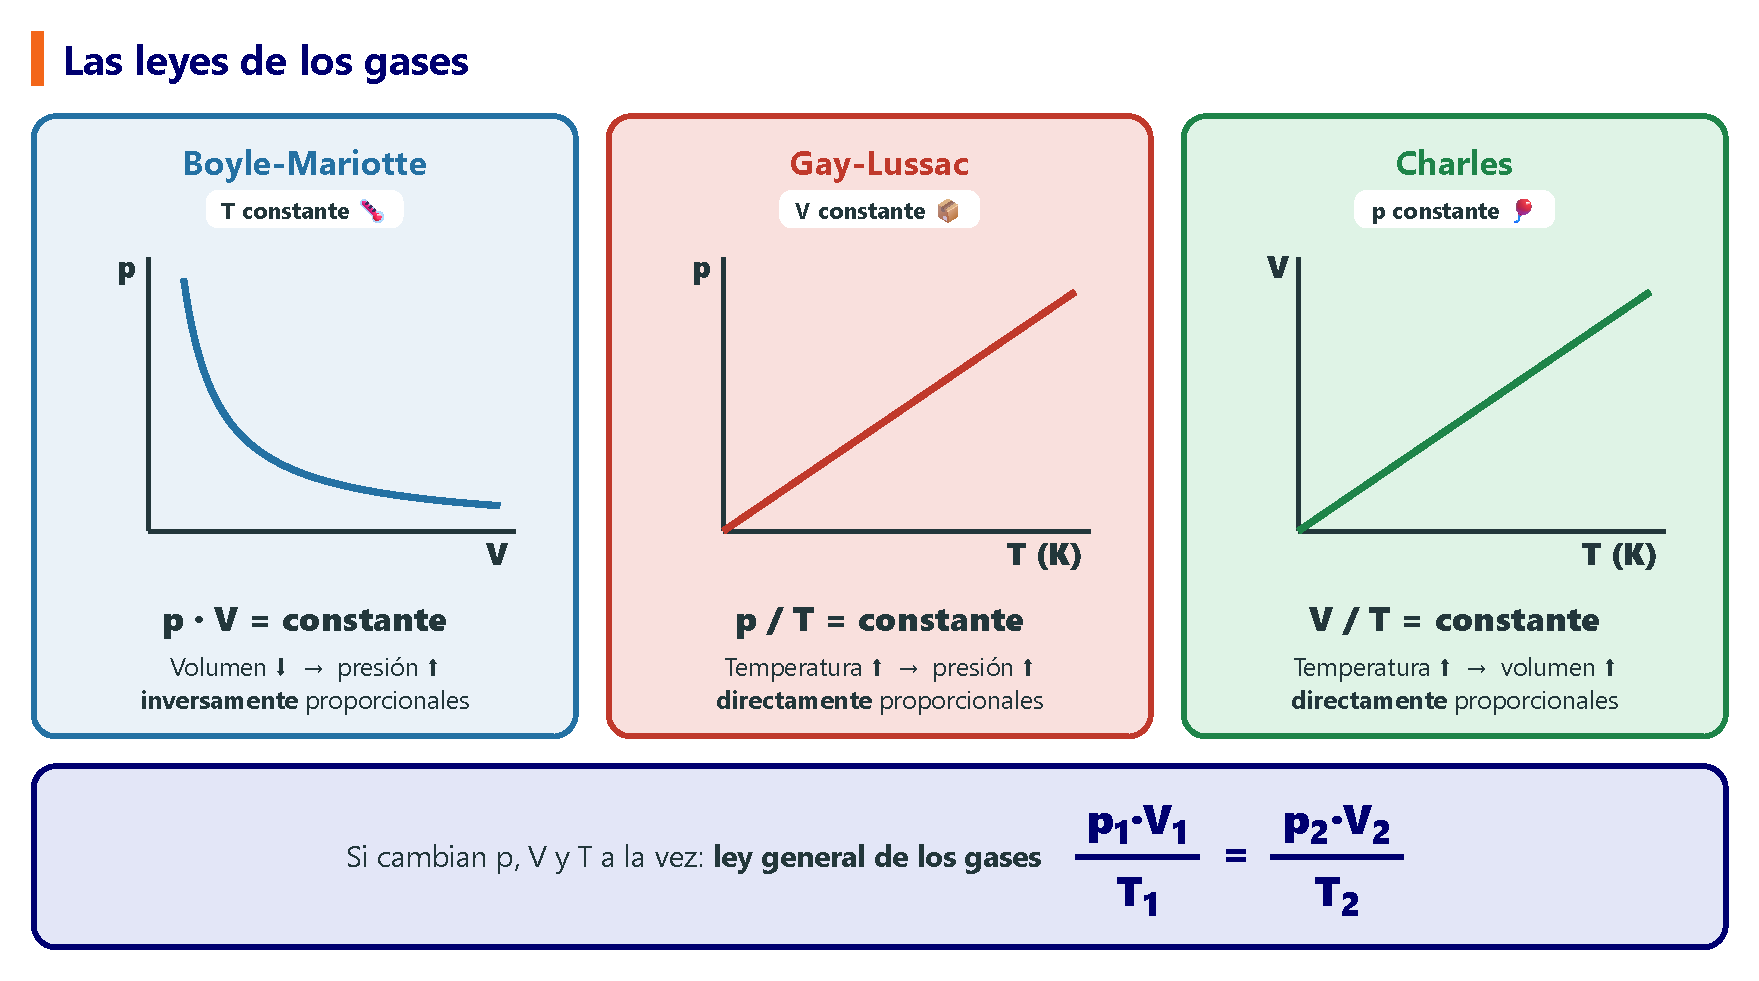
\includegraphics[width=\textwidth]{FigurasSVG/Unit_2_State_of_Matter/pdf/gas_laws_es.pdf}
    \caption{Las tres leyes de los gases y la ley general de los gases.}
    \label{fig:u2_gas_laws}
\end{figure}

\begin{table}[H]
    \centering
    \renewcommand{\arraystretch}{2}
    \begin{tabular}{lccc}
        \toprule
        \textbf{Ley} & \textbf{Constante} & \textbf{Ecuación} & \textbf{Relación} \\
        \midrule
        Boyle-Mariotte & \(T\) & \(p_1 \cdot V_1 = p_2 \cdot V_2\) & inversamente proporcionales \\
        Gay-Lussac & \(V\) & \(\dfrac{p_1}{T_1} = \dfrac{p_2}{T_2}\) & directamente proporcionales \\
        Charles & \(p\) & \(\dfrac{V_1}{T_1} = \dfrac{V_2}{T_2}\) & directamente proporcionales \\
        \bottomrule
    \end{tabular}
    \caption{Las leyes de los gases.}
    \label{tab:u2_gas_laws}
\end{table}

\begin{impt}
    \negsubro{¿Cómo sabemos qué ley hay que usar?} Buscamos la magnitud que \textbf{no} cambia (la que se mantiene \textbf{constante}):
    \begin{itemize}
        \item \(T\) constante \(\to\) \textbf{ley de Boyle-Mariotte}.
        \item \(V\) constante \(\to\) \textbf{ley de Gay-Lussac}.
        \item \(p\) constante \(\to\) \textbf{ley de Charles}.
    \end{itemize}
    El método completo, paso a paso, está en el apartado \emph{Ejercicios de leyes de los gases}.
\end{impt}

%------------------------------------------------

\subsection{Ley de Boyle-Mariotte (temperatura constante)}

\negsubro{¿Qué nos dice esta ley?} Coge una bomba de bicicleta, tapa el agujero con el dedo y empuja el mango. Cuanto más empujas (cuanto \textbf{menor es el volumen}), con más fuerza empuja el aire contra tu mano (\textbf{mayor es la presión}).

¿Por qué ocurre esto? Si la temperatura de un gas no cambia, sus partículas siguen moviéndose a la misma velocidad. Cuando \textbf{comprimimos} el gas, las partículas tienen menos espacio, así que chocan contra las paredes del recipiente \textbf{más a menudo}: la \textbf{presión aumenta}. Si dejamos que el gas se \textbf{expanda}, las partículas tienen más espacio, chocan contra las paredes con menos frecuencia y la presión \textbf{disminuye}.

Decimos que la presión y el volumen son \textbf{inversamente proporcionales}: cuando uno \textbf{sube}, el otro \textbf{baja}. Si el volumen se reduce a la mitad, la presión se duplica; si el volumen se duplica, la presión se reduce a la mitad.

\begin{definition}[Ley de Boyle-Mariotte]
    A temperatura constante, el producto de la presión por el volumen de un gas se mantiene constante:
    \begin{equation*}
        p_1 \cdot V_1 = p_2 \cdot V_2
    \end{equation*}
\end{definition}

\begin{figure}[H]
    \centering
    % [FIGURA ORIGINAL] \includegraphics[width=\textwidth]{Unit_2/boyle_law}
    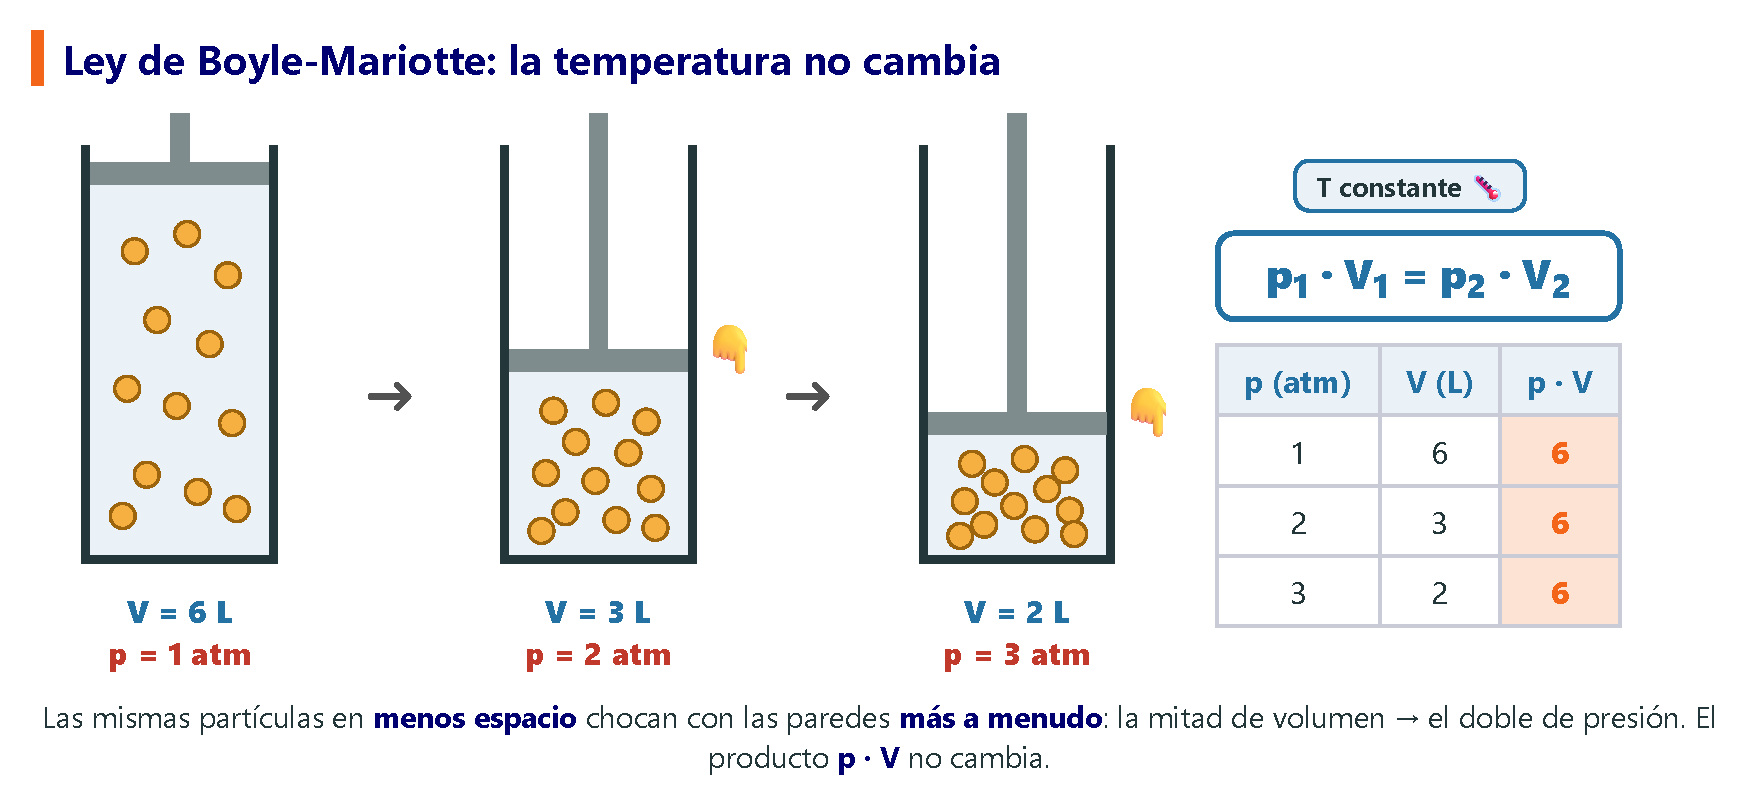
\includegraphics[width=\textwidth]{FigurasSVG/Unit_2_State_of_Matter/pdf/boyle_law_es.pdf}
    \caption{Ley de Boyle-Mariotte: a temperatura constante, cuando el volumen disminuye la presión aumenta, y \(p \cdot V\) no cambia.}
    \label{fig:u2_boyle_law}
\end{figure}

\begin{example}
    \textbf{En un recipiente de \qty{3}{\litre}, un gas ejerce una presión de \qty{2}{\atmospher} a \qty{60}{\celsius}. ¿Cuál será su volumen si la presión se duplica hasta \qty{4}{\atmospher} y la temperatura no cambia?}
    \begin{enumerate}[label=\numberballmDarkTeal]
        \item Datos: \(p_1 = \qty{2}{\atmospher}\), \(V_1 = \qty{3}{\litre}\), \(p_2 = \qty{4}{\atmospher}\). Incógnita: \(\underline{V_2}\).
        \item \(T\) es constante \(\to\) \textbf{ley de Boyle-Mariotte}: \(p_1 \cdot V_1 = p_2 \cdot V_2\).
        \item Despejamos \(V_2\) y calculamos:
        \(\;V_2 = \dfrac{p_1 \cdot V_1}{p_2} = \dfrac{\qty{2}{\atmospher} \cdot \qty{3}{\litre}}{\qty{4}{\atmospher}} = \textcolor{red}{\qty{1.5}{\litre}}\)
    \end{enumerate}
    La presión se duplica, así que el volumen se reduce a la mitad: ¡tiene sentido!
\end{example}

\begin{exercise}
    En un recipiente de \qty{3}{\litre}, el nitrógeno ejerce una presión de \qty{4}{\atmospher}. ¿Cuál será la presión si el volumen del recipiente se duplica y la temperatura no cambia?
    \begin{solu}
        \(T\) constante \(\to\) ley de Boyle-Mariotte: \(p_1 \cdot V_1 = p_2 \cdot V_2\). \\
        \(p_2 = \dfrac{p_1 \cdot V_1}{V_2} = \dfrac{\qty{4}{\atmospher} \cdot \qty{3}{\litre}}{\qty{6}{\litre}} = \qty{2}{\atmospher}\).
    \end{solu}
\end{exercise}

\begin{exercise}
    \qty{22.5}{\litre} de nitrógeno a \qty{748}{\mmhg} se llevan, a temperatura constante, hasta una presión de \qty{725}{\mmhg}. ¿Cuál es el nuevo volumen?
    \begin{solu}
        \(T\) constante \(\to\) ley de Boyle-Mariotte: \(p_1 \cdot V_1 = p_2 \cdot V_2\). \\
        \(V_2 = \dfrac{p_1 \cdot V_1}{p_2} = \dfrac{\qty{748}{\mmhg} \cdot \qty{22.5}{\litre}}{\qty{725}{\mmhg}} \approx \qty{23.2}{\litre}\).
    \end{solu}
\end{exercise}

\subsubsection{Cómo despejar cada magnitud en la ley de Boyle-Mariotte}

En un ejercicio, la incógnita puede ser cualquiera de las cuatro magnitudes. Siempre partimos de la ley, \(p_1 \cdot V_1 = p_2 \cdot V_2\), y dejamos la incógnita \textbf{sola}. Igual que hicimos con la densidad, hacemos la \textbf{misma operación en los dos miembros}: si la incógnita está \textbf{multiplicada} por una magnitud, \textbf{dividimos} los dos miembros entre esa magnitud (o, con el atajo, lo que está \textbf{multiplicando} pasa al otro lado \textbf{dividiendo}).

\begin{figure}[H]
    \centering
    % [FIGURA ORIGINAL] \includegraphics[width=\textwidth]{Unit_2/boyle_isolate}
    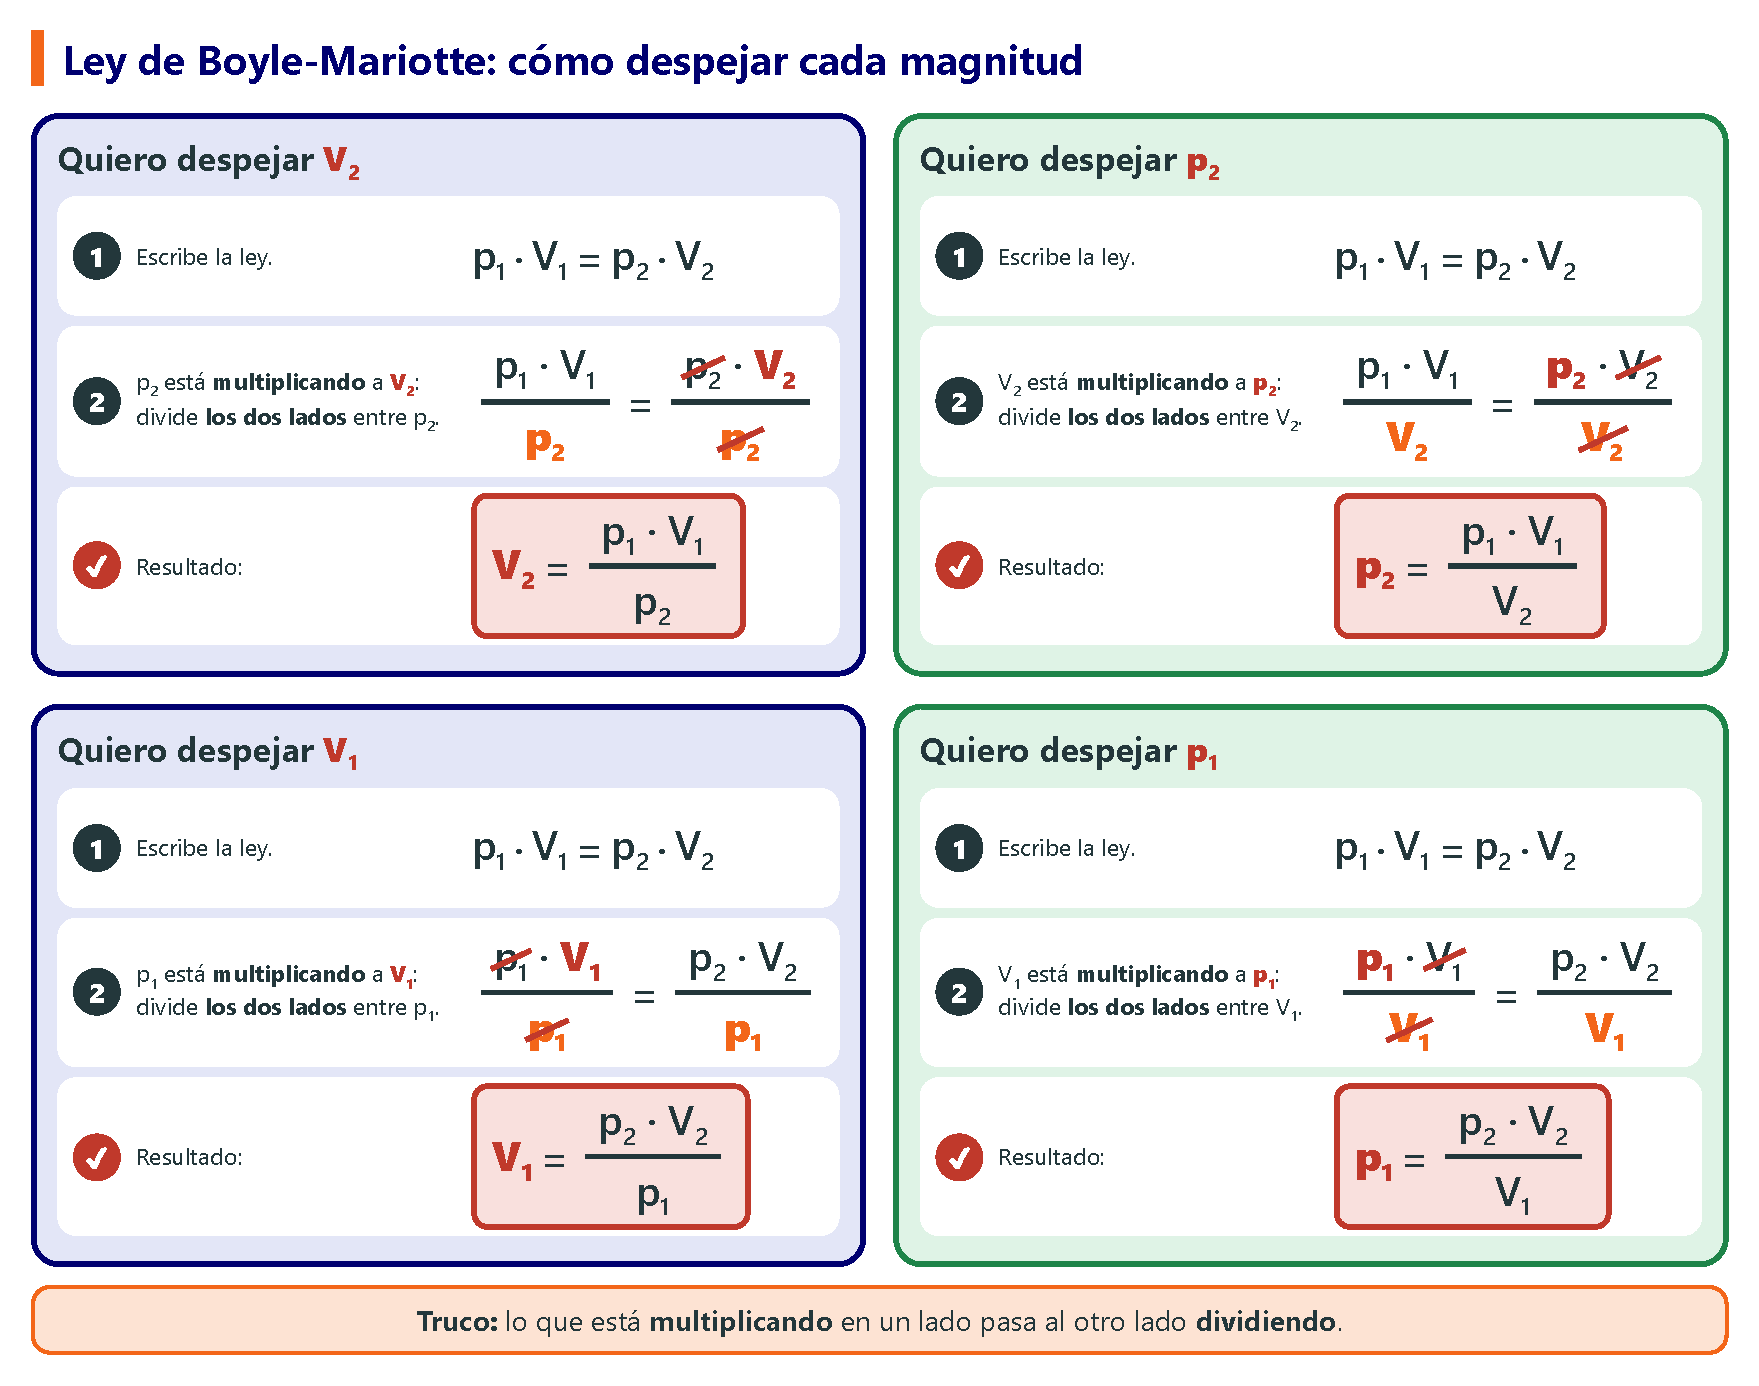
\includegraphics[width=\textwidth]{FigurasSVG/Unit_2_State_of_Matter/pdf/boyle_isolate_es.pdf}
    \caption{Cómo despejar \(V_2\), \(p_2\), \(V_1\) y \(p_1\) en la ley de Boyle-Mariotte, paso a paso.}
    \label{fig:u2_boyle_isolate}
\end{figure}

\begin{itemize}
    \item \textbf{Incógnita \(V_2\)}: \(p_2\) está multiplicando a \(V_2\), así que dividimos los dos miembros entre \(p_2\):
    \(\;\dfrac{p_1 \cdot V_1}{p_2} = \dfrac{\cancelred{p_2} \cdot V_2}{\cancelred{p_2}} \;\Rightarrow\; \textcolor{red}{V_2 = \dfrac{p_1 \cdot V_1}{p_2}}\)
    \item \textbf{Incógnita \(p_2\)}: \(V_2\) está multiplicando a \(p_2\), así que dividimos los dos miembros entre \(V_2\):
    \(\;\dfrac{p_1 \cdot V_1}{V_2} = \dfrac{p_2 \cdot \cancelred{V_2}}{\cancelred{V_2}} \;\Rightarrow\; \textcolor{red}{p_2 = \dfrac{p_1 \cdot V_1}{V_2}}\)
    \item \textbf{Incógnita \(V_1\)}: \(p_1\) está multiplicando a \(V_1\), así que dividimos los dos miembros entre \(p_1\):
    \(\;\dfrac{\cancelred{p_1} \cdot V_1}{\cancelred{p_1}} = \dfrac{p_2 \cdot V_2}{p_1} \;\Rightarrow\; \textcolor{red}{V_1 = \dfrac{p_2 \cdot V_2}{p_1}}\)
    \item \textbf{Incógnita \(p_1\)}: \(V_1\) está multiplicando a \(p_1\), así que dividimos los dos miembros entre \(V_1\):
    \(\;\dfrac{p_1 \cdot \cancelred{V_1}}{\cancelred{V_1}} = \dfrac{p_2 \cdot V_2}{V_1} \;\Rightarrow\; \textcolor{red}{p_1 = \dfrac{p_2 \cdot V_2}{V_1}}\)
\end{itemize}

%------------------------------------------------

\subsection{Ley de Gay-Lussac (volumen constante)}

\negsubro{¿Qué nos dice esta ley?} ¿Te has fijado en que los botes de espray llevan un aviso: «No dejar al sol ni cerca del fuego»? El bote es de metal, así que el gas de su interior no puede cambiar de volumen. Si se \textbf{calienta}, la \textbf{presión} del gas \textbf{aumenta} tanto que el bote podría explotar.

¿Por qué ocurre esto? Si un gas está dentro de un recipiente cerrado y rígido, su volumen no puede cambiar. Cuando lo \textbf{calentamos}, sus partículas se mueven \textbf{más deprisa} y chocan contra las paredes \textbf{con más fuerza y más a menudo}: la \textbf{presión aumenta}. Cuando lo enfriamos, las partículas se mueven más despacio y la presión disminuye.

Decimos que la presión y la temperatura (en kelvin) son \textbf{directamente proporcionales}: cuando una \textbf{sube}, la otra también \textbf{sube}. Si la temperatura en kelvin se duplica, la presión también se duplica.

\begin{definition}[Ley de Gay-Lussac]
    A volumen constante, la presión de un gas dividida entre su temperatura en kelvin se mantiene constante:
    \begin{equation*}
        \dfrac{p_1}{T_1} = \dfrac{p_2}{T_2}
    \end{equation*}
\end{definition}

\begin{figure}[H]
    \centering
    % [FIGURA ORIGINAL] \includegraphics[width=\textwidth]{Unit_2/gay_lussac_law}
    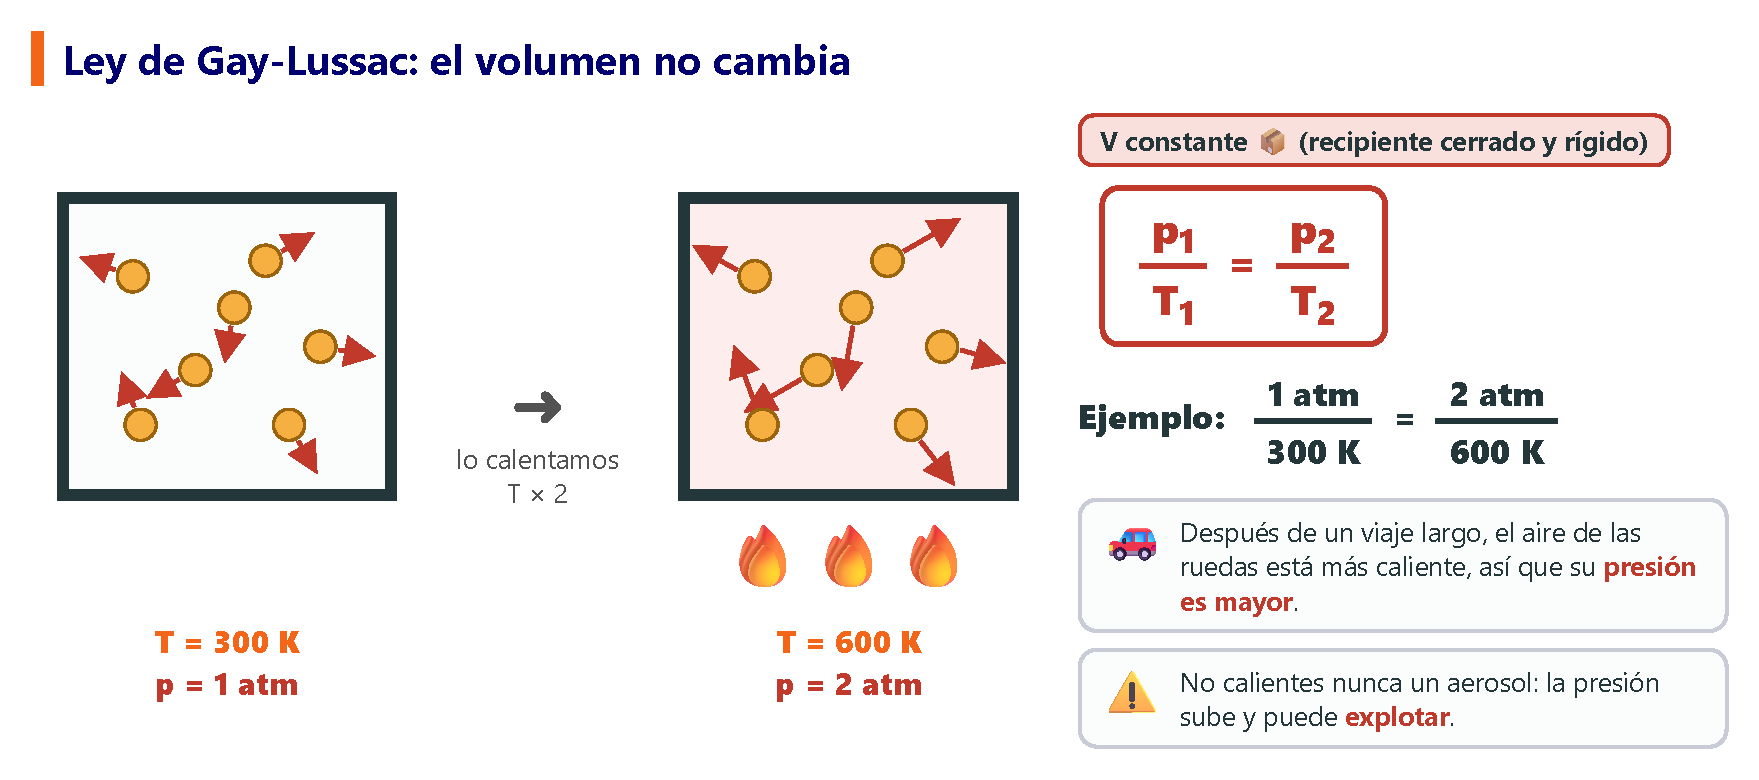
\includegraphics[width=\textwidth]{FigurasSVG/Unit_2_State_of_Matter/pdf/gay_lussac_law_es.pdf}
    \caption{Ley de Gay-Lussac: en un recipiente rígido, si la temperatura en kelvin se duplica, la presión también se duplica.}
    \label{fig:u2_gay_lussac_law}
\end{figure}

\begin{example}
    \textbf{Un recipiente cerrado con gas está al principio a \qty{0.500}{\atmospher} y \qty{25.0}{\celsius}. ¿Cuál será la presión a \qty{125.0}{\celsius}?}
    \begin{enumerate}[label=\numberballmDarkTeal]
        \item Datos: \(p_1 = \qty{0.500}{\atmospher}\), \(T_1 = 25 + 273 = \qty{298}{\kelvin}\), \(T_2 = 125 + 273 = \qty{398}{\kelvin}\). Incógnita: \(\underline{p_2}\).
        \item El recipiente está cerrado, así que \(V\) es constante \(\to\) \textbf{ley de Gay-Lussac}: \(\dfrac{p_1}{T_1} = \dfrac{p_2}{T_2}\).
        \item Despejamos \(p_2\) y calculamos:
        \(\;p_2 = \dfrac{p_1 \cdot T_2}{T_1} = \dfrac{\qty{0.500}{\atmospher} \cdot \qty{398}{\kelvin}}{\qty{298}{\kelvin}} \approx \textcolor{red}{\qty{0.668}{\atmospher}}\)
    \end{enumerate}
    La temperatura sube, así que la presión también sube: ¡tiene sentido!
\end{example}

\begin{exercise}
    En un recipiente de \qty{10}{\litre}, el oxígeno ejerce una presión de \qty{4}{\atmospher} a \qty{20}{\celsius}. ¿Cuál será la presión si la temperatura sube a \qty{40}{\celsius} y el volumen no cambia?
    \begin{solu}
        \(V\) constante \(\to\) ley de Gay-Lussac: \(\dfrac{p_1}{T_1} = \dfrac{p_2}{T_2}\). \\
        En kelvin: \(T_1 = 20 + 273 = \qty{293}{\kelvin}\); \(T_2 = 40 + 273 = \qty{313}{\kelvin}\). \\
        \(p_2 = \dfrac{p_1 \cdot T_2}{T_1} = \dfrac{\qty{4}{\atmospher} \cdot \qty{313}{\kelvin}}{\qty{293}{\kelvin}} \approx \qty{4.27}{\atmospher}\).
    \end{solu}
\end{exercise}

\begin{exercise}
    Un gas se enfría de \qty{323}{\kelvin} a \qty{273}{\kelvin} manteniendo constante su volumen. ¿Cuál es la presión final si la presión inicial era de \qty{750.0}{\mmhg}?
    \begin{solu}
        \(V\) constante \(\to\) ley de Gay-Lussac: \(\dfrac{p_1}{T_1} = \dfrac{p_2}{T_2}\). \\
        \(p_2 = \dfrac{p_1 \cdot T_2}{T_1} = \dfrac{\qty{750.0}{\mmhg} \cdot \qty{273}{\kelvin}}{\qty{323}{\kelvin}} \approx \qty{634}{\mmhg}\).
    \end{solu}
\end{exercise}

\subsubsection{Cómo despejar cada magnitud en la ley de Gay-Lussac}

Siempre partimos de la ley, \(\dfrac{p_1}{T_1} = \dfrac{p_2}{T_2}\). Aquí las magnitudes están dentro de fracciones, así que lo hacemos en dos pasos:
\begin{enumerate}[label=\numberballmDarkTeal]
    \item \textbf{Quitamos las fracciones (multiplicación en cruz).} \(T_1\) está \textbf{dividiendo} a la izquierda, así que pasa a la derecha \textbf{multiplicando}; \(T_2\) está \textbf{dividiendo} a la derecha, así que pasa a la izquierda \textbf{multiplicando}:
    \begin{equation*}
        \dfrac{p_1}{T_1} = \dfrac{p_2}{T_2} \quad\Longrightarrow\quad p_1 \cdot T_2 = p_2 \cdot T_1
    \end{equation*}
    \item \textbf{Despejamos la incógnita}: la magnitud que está \textbf{multiplicando} a la incógnita pasa al otro lado \textbf{dividiendo} (dividimos los dos miembros entre ella).
\end{enumerate}

\begin{figure}[H]
    \centering
    % [FIGURA ORIGINAL] \includegraphics[width=\textwidth]{Unit_2/gay_lussac_isolate}
    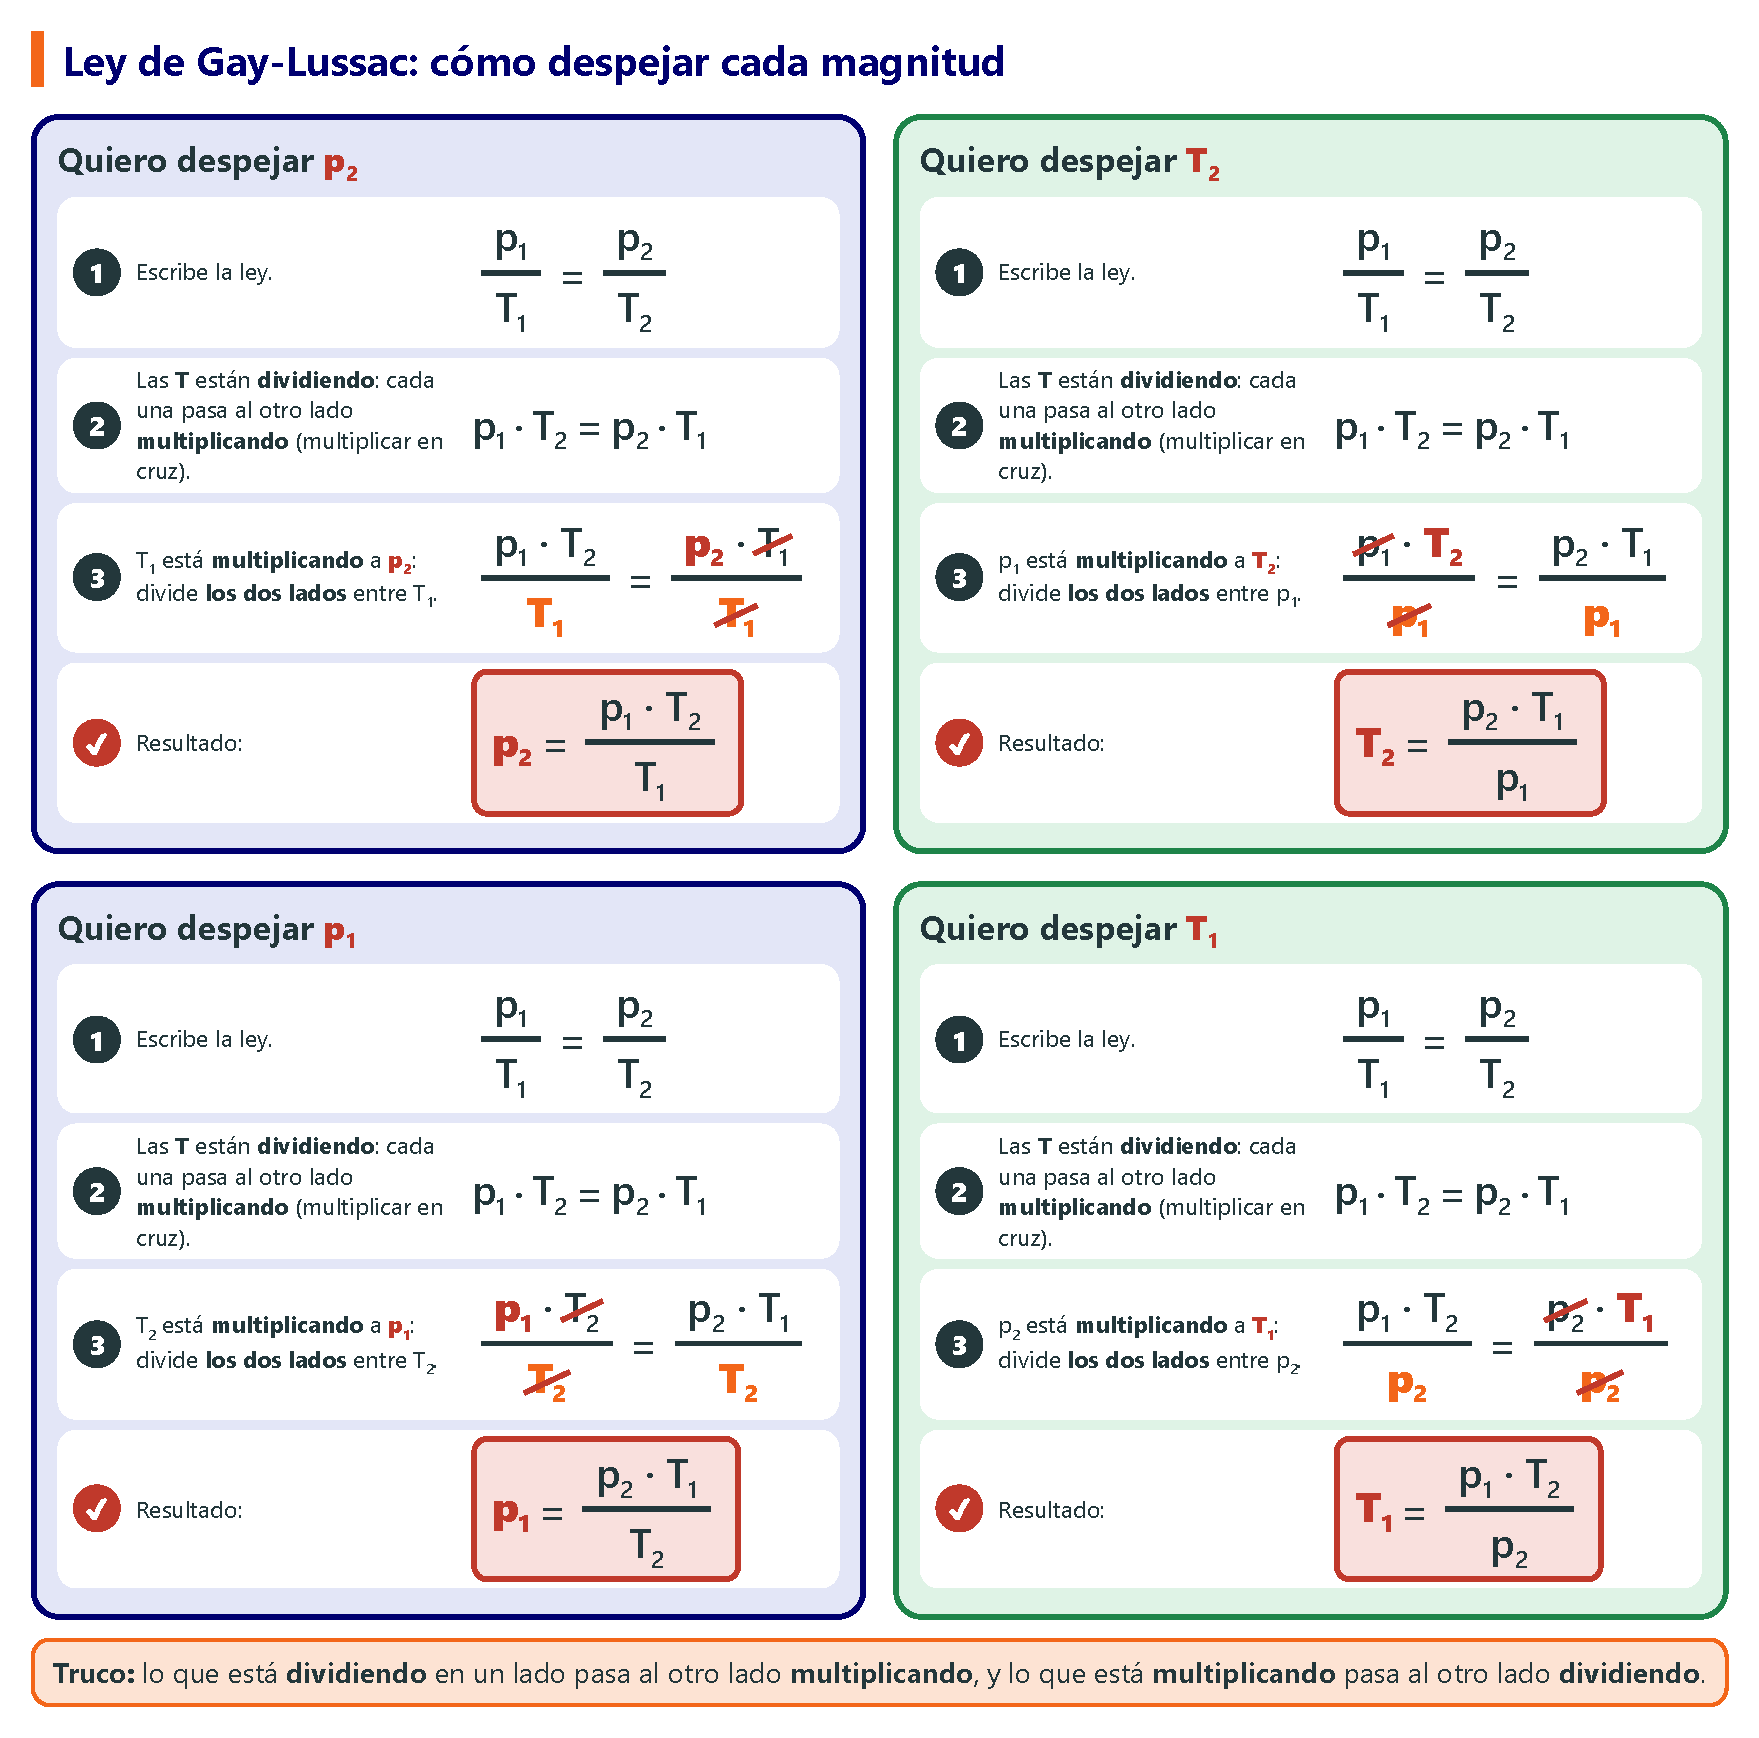
\includegraphics[width=\textwidth]{FigurasSVG/Unit_2_State_of_Matter/pdf/gay_lussac_isolate_es.pdf}
    \caption{Cómo despejar las cuatro magnitudes en la ley de Gay-Lussac, paso a paso.}
    \label{fig:u2_gay_lussac_isolate}
\end{figure}

Partiendo de \(p_1 \cdot T_2 = p_2 \cdot T_1\):
\begin{itemize}
    \item \textbf{Incógnita \(p_2\)}: dividimos los dos miembros entre \(T_1\):
    \(\;\dfrac{p_1 \cdot T_2}{T_1} = \dfrac{p_2 \cdot \cancelred{T_1}}{\cancelred{T_1}} \;\Rightarrow\; \textcolor{red}{p_2 = \dfrac{p_1 \cdot T_2}{T_1}}\)
    \item \textbf{Incógnita \(T_2\)}: dividimos los dos miembros entre \(p_1\):
    \(\;\dfrac{\cancelred{p_1} \cdot T_2}{\cancelred{p_1}} = \dfrac{p_2 \cdot T_1}{p_1} \;\Rightarrow\; \textcolor{red}{T_2 = \dfrac{p_2 \cdot T_1}{p_1}}\)
    \item \textbf{Incógnita \(p_1\)}: dividimos los dos miembros entre \(T_2\):
    \(\;\dfrac{p_1 \cdot \cancelred{T_2}}{\cancelred{T_2}} = \dfrac{p_2 \cdot T_1}{T_2} \;\Rightarrow\; \textcolor{red}{p_1 = \dfrac{p_2 \cdot T_1}{T_2}}\)
    \item \textbf{Incógnita \(T_1\)}: dividimos los dos miembros entre \(p_2\):
    \(\;\dfrac{p_1 \cdot T_2}{p_2} = \dfrac{\cancelred{p_2} \cdot T_1}{\cancelred{p_2}} \;\Rightarrow\; \textcolor{red}{T_1 = \dfrac{p_1 \cdot T_2}{p_2}}\)
\end{itemize}

%------------------------------------------------

\subsection{Ley de Charles (presión constante)}

\negsubro{¿Qué nos dice esta ley?} Infla un globo y mételo en el congelador: al cabo de un rato parece más pequeño y arrugado. Sácalo y déjalo al sol: vuelve a hacerse grande. Cuanto \textbf{más frío} está el gas, \textbf{menor es su volumen}; cuanto \textbf{más caliente} está, \textbf{mayor es su volumen}.

¿Por qué ocurre esto? Aquí la presión del gas no cambia (un globo, o una jeringuilla cuyo émbolo se puede mover libremente). Cuando \textbf{calentamos} el gas, sus partículas se mueven \textbf{más deprisa} y empujan las paredes \textbf{hacia fuera}: el gas se \textbf{expande} (su volumen aumenta). Cuando lo enfriamos, las partículas se mueven más despacio y el gas se \textbf{contrae}.

Decimos que el volumen y la temperatura (en kelvin) son \textbf{directamente proporcionales}: cuando uno \textbf{sube}, el otro también \textbf{sube}. Si la temperatura en kelvin se duplica, el volumen también se duplica.

\begin{definition}[Ley de Charles]
    A presión constante, el volumen de un gas dividido entre su temperatura en kelvin se mantiene constante:
    \begin{equation*}
        \dfrac{V_1}{T_1} = \dfrac{V_2}{T_2}
    \end{equation*}
\end{definition}

\begin{figure}[H]
    \centering
    % [FIGURA ORIGINAL] \includegraphics[width=\textwidth]{Unit_2/charles_law}
    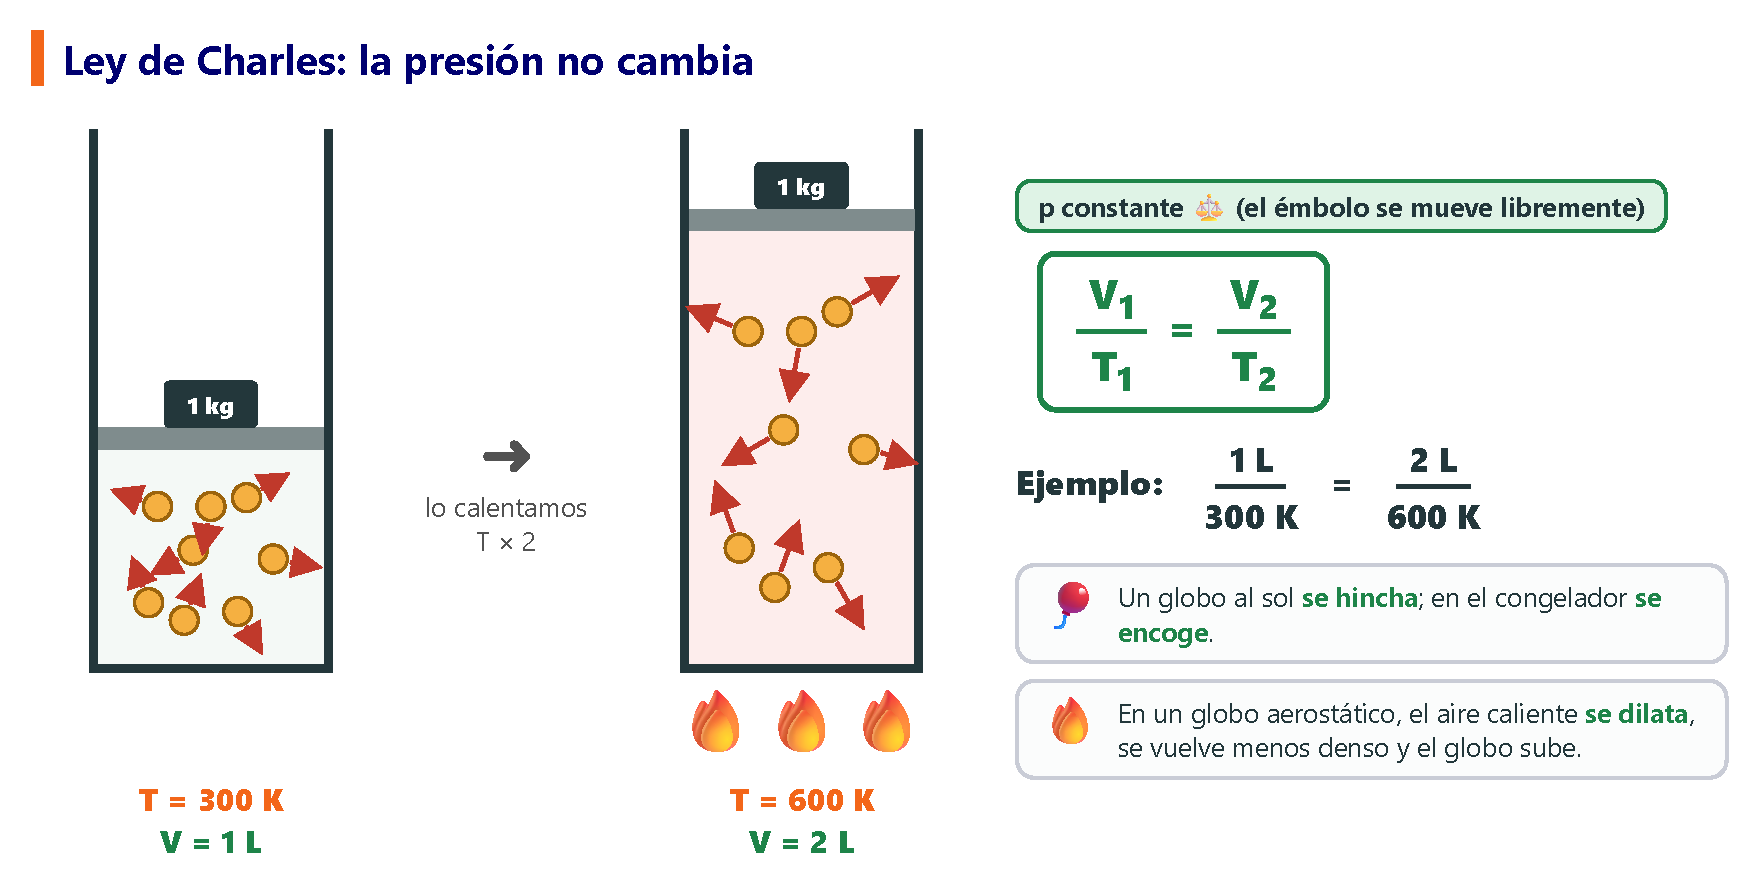
\includegraphics[width=\textwidth]{FigurasSVG/Unit_2_State_of_Matter/pdf/charles_law_es.pdf}
    \caption{Ley de Charles: con un émbolo libre la presión no cambia, y si la temperatura en kelvin se duplica, el volumen también se duplica.}
    \label{fig:u2_charles_law}
\end{figure}

\begin{example}
    \textbf{Un gas ocupa \qty{900.0}{\mL} a \qty{27.0}{\celsius}. ¿Cuál es su volumen a \qty{132.0}{\celsius} si la presión no cambia?}
    \begin{enumerate}[label=\numberballmDarkTeal]
        \item Datos: \(V_1 = \qty{900.0}{\mL}\), \(T_1 = 27 + 273 = \qty{300}{\kelvin}\), \(T_2 = 132 + 273 = \qty{405}{\kelvin}\). Incógnita: \(\underline{V_2}\).
        \item \(p\) es constante \(\to\) \textbf{ley de Charles}: \(\dfrac{V_1}{T_1} = \dfrac{V_2}{T_2}\).
        \item Despejamos \(V_2\) y calculamos:
        \(\;V_2 = \dfrac{V_1 \cdot T_2}{T_1} = \dfrac{\qty{900.0}{\mL} \cdot \qty{405}{\kelvin}}{\qty{300}{\kelvin}} = \textcolor{red}{\qty{1215}{\mL}}\)
    \end{enumerate}
    La temperatura sube, así que el gas se expande: ¡tiene sentido!
\end{example}

\begin{exercise}
    Un gas ocupa \qty{2}{\litre} a \qty{300}{\kelvin}. ¿Qué volumen ocupará si la temperatura sube a \qty{450}{\kelvin} sin que cambie la presión?
    \begin{solu}
        \(p\) constante \(\to\) ley de Charles: \(\dfrac{V_1}{T_1} = \dfrac{V_2}{T_2}\). \\
        \(V_2 = \dfrac{V_1 \cdot T_2}{T_1} = \dfrac{\qty{2}{\litre} \cdot \qty{450}{\kelvin}}{\qty{300}{\kelvin}} = \qty{3}{\litre}\).
    \end{solu}
\end{exercise}

\begin{exercise}
    Se recogen \qty{5.00}{\litre} de un gas a \qty{100}{\kelvin} y después se deja que se expanda hasta \qty{20.0}{\litre}. ¿Cuál debe ser la nueva temperatura para que la presión no cambie?
    \begin{solu}
        \(p\) constante \(\to\) ley de Charles: \(\dfrac{V_1}{T_1} = \dfrac{V_2}{T_2}\). \\
        \(T_2 = \dfrac{V_2 \cdot T_1}{V_1} = \dfrac{\qty{20.0}{\litre} \cdot \qty{100}{\kelvin}}{\qty{5.00}{\litre}} = \qty{400}{\kelvin}\).
    \end{solu}
\end{exercise}

\subsubsection{Cómo despejar cada magnitud en la ley de Charles}

Siempre partimos de la ley, \(\dfrac{V_1}{T_1} = \dfrac{V_2}{T_2}\). Aquí las magnitudes están dentro de fracciones, así que lo hacemos en dos pasos:
\begin{enumerate}[label=\numberballmDarkTeal]
    \item \textbf{Quitamos las fracciones (multiplicación en cruz).} \(T_1\) está \textbf{dividiendo} a la izquierda, así que pasa a la derecha \textbf{multiplicando}; \(T_2\) está \textbf{dividiendo} a la derecha, así que pasa a la izquierda \textbf{multiplicando}:
    \begin{equation*}
        \dfrac{V_1}{T_1} = \dfrac{V_2}{T_2} \quad\Longrightarrow\quad V_1 \cdot T_2 = V_2 \cdot T_1
    \end{equation*}
    \item \textbf{Despejamos la incógnita}: la magnitud que está \textbf{multiplicando} a la incógnita pasa al otro lado \textbf{dividiendo} (dividimos los dos miembros entre ella).
\end{enumerate}

\begin{figure}[H]
    \centering
    % [FIGURA ORIGINAL] \includegraphics[width=\textwidth]{Unit_2/charles_isolate}
    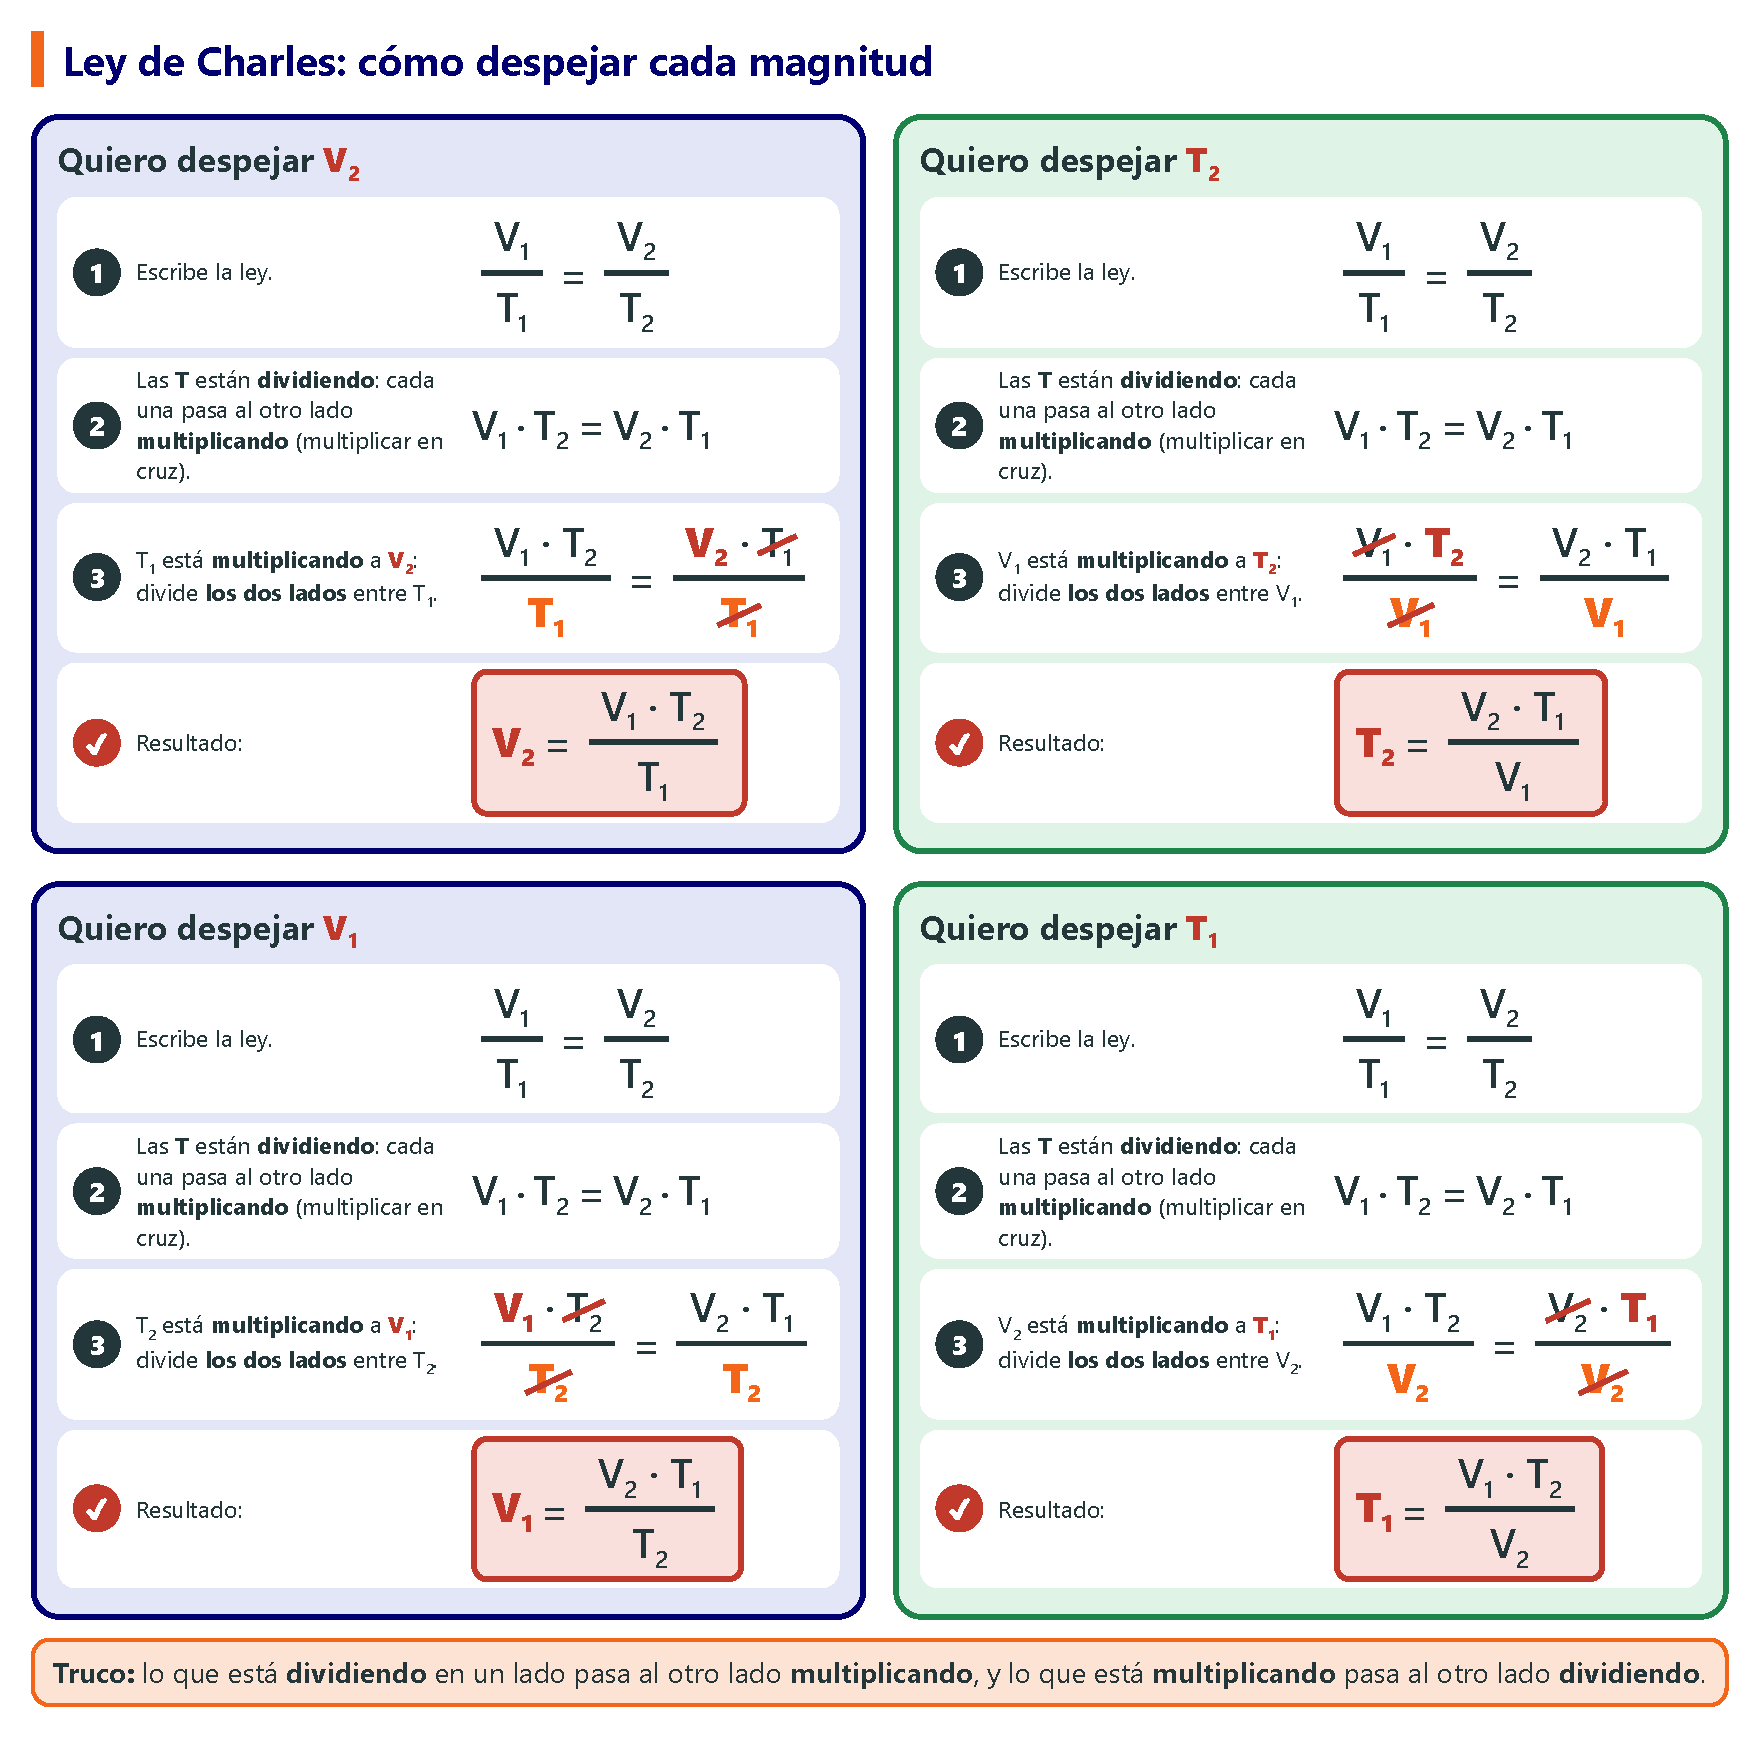
\includegraphics[width=\textwidth]{FigurasSVG/Unit_2_State_of_Matter/pdf/charles_isolate_es.pdf}
    \caption{Cómo despejar las cuatro magnitudes en la ley de Charles, paso a paso.}
    \label{fig:u2_charles_isolate}
\end{figure}

Partiendo de \(V_1 \cdot T_2 = V_2 \cdot T_1\):
\begin{itemize}
    \item \textbf{Incógnita \(V_2\)}: dividimos los dos miembros entre \(T_1\):
    \(\;\dfrac{V_1 \cdot T_2}{T_1} = \dfrac{V_2 \cdot \cancelred{T_1}}{\cancelred{T_1}} \;\Rightarrow\; \textcolor{red}{V_2 = \dfrac{V_1 \cdot T_2}{T_1}}\)
    \item \textbf{Incógnita \(T_2\)}: dividimos los dos miembros entre \(V_1\):
    \(\;\dfrac{\cancelred{V_1} \cdot T_2}{\cancelred{V_1}} = \dfrac{V_2 \cdot T_1}{V_1} \;\Rightarrow\; \textcolor{red}{T_2 = \dfrac{V_2 \cdot T_1}{V_1}}\)
    \item \textbf{Incógnita \(V_1\)}: dividimos los dos miembros entre \(T_2\):
    \(\;\dfrac{V_1 \cdot \cancelred{T_2}}{\cancelred{T_2}} = \dfrac{V_2 \cdot T_1}{T_2} \;\Rightarrow\; \textcolor{red}{V_1 = \dfrac{V_2 \cdot T_1}{T_2}}\)
    \item \textbf{Incógnita \(T_1\)}: dividimos los dos miembros entre \(V_2\):
    \(\;\dfrac{V_1 \cdot T_2}{V_2} = \dfrac{\cancelred{V_2} \cdot T_1}{\cancelred{V_2}} \;\Rightarrow\; \textcolor{red}{T_1 = \dfrac{V_1 \cdot T_2}{V_2}}\)
\end{itemize}

%------------------------------------------------

\subsection{Ejercicios de leyes de los gases}

En estos ejercicios las leyes aparecen mezcladas. Para resolverlos bien, sigue siempre el mismo procedimiento:

\negsubro{Método, paso a paso}:
\begin{enumerate}[label=\numberballmDarkTeal]
    \item \textbf{Lee} el ejercicio \textbf{una vez}, para entender qué está pasando.
    \item \textbf{Lee} el ejercicio \textbf{una segunda vez}, buscando los números y sus unidades.
    \item Dibuja una \textbf{tabla} con dos columnas: \textbf{Datos} e \textbf{Incógnita}.
    \item Escribe los \textbf{datos} que te da el ejercicio, indicando si cada uno corresponde al \textbf{principio (1)} o al \textbf{final (2)}: \(p_1\), \(V_1\), \(T_1\), \(p_2\)\ldots{} Pasa las temperaturas a \textbf{kelvin}.
    \item En la columna \textbf{Incógnita}, escribe lo que te pide el ejercicio.
    \item Busca la magnitud que se mantiene \textbf{constante}. Te indica qué ley tienes que usar: escribe su \textbf{nombre}.
    \item Escribe la \textbf{fórmula} de esa ley.
    \item \textbf{Despeja} la incógnita en la fórmula.
    \item \textbf{Sustituye} cada magnitud por su número (con sus unidades), \textbf{calcula} y comprueba que el resultado tiene sentido.
\end{enumerate}

\begin{figure}[H]
    \centering
    % [FIGURA ORIGINAL] \includegraphics[width=\textwidth]{Unit_2/gas_law_method}
    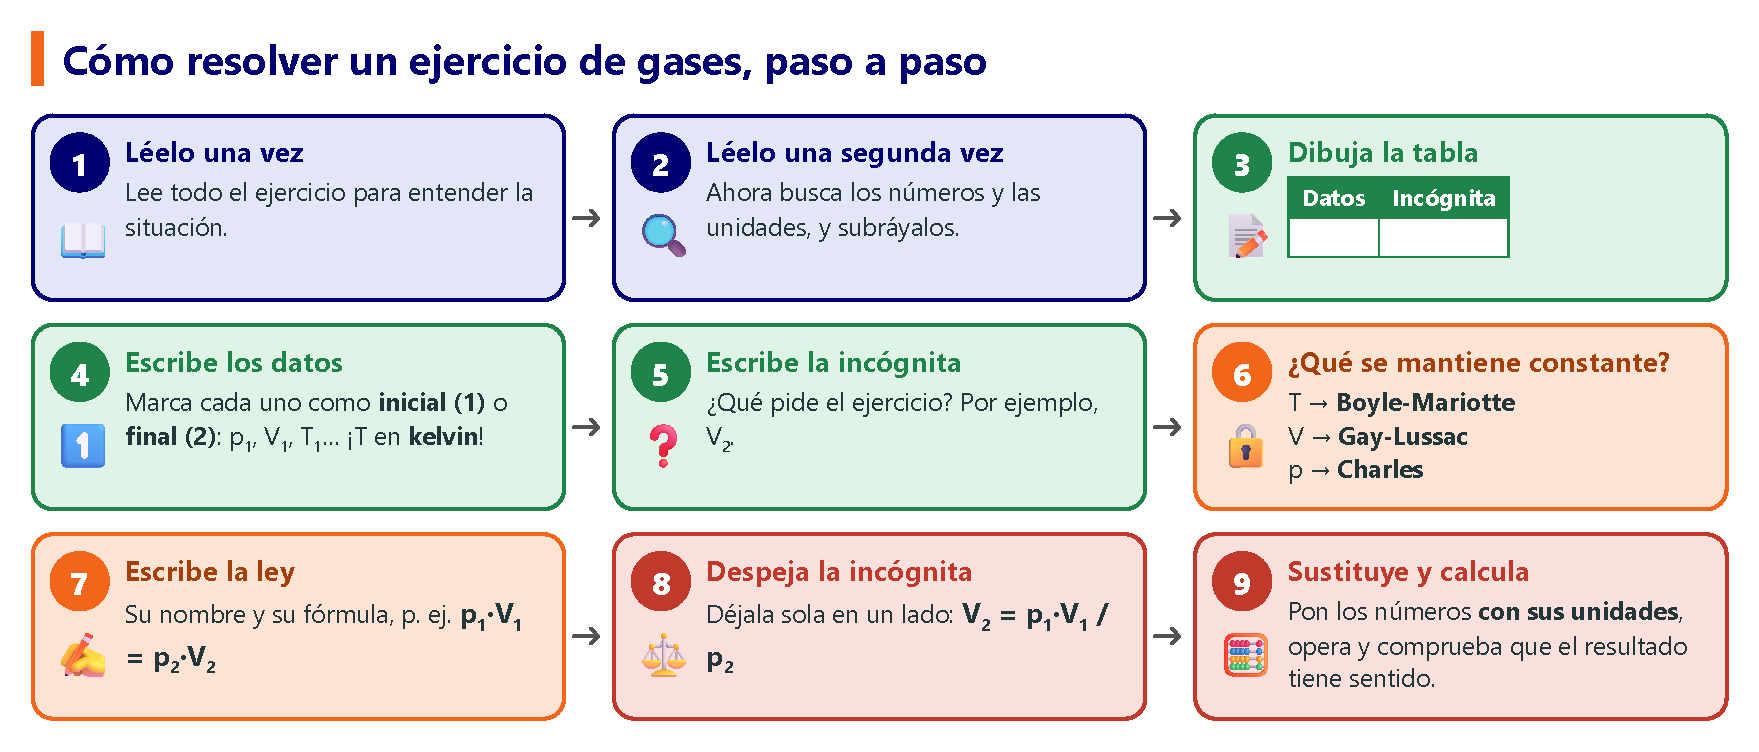
\includegraphics[width=\textwidth]{FigurasSVG/Unit_2_State_of_Matter/pdf/gas_law_method_es.pdf}
    \caption{Los nueve pasos para resolver un ejercicio de leyes de los gases.}
    \label{fig:u2_gas_law_method}
\end{figure}

\begin{example}
    \textbf{Un gas ocupa \qty{2.0}{\litre} a \qty{27}{\celsius}. Se calienta hasta \qty{127}{\celsius} sin cambiar su presión. ¿Cuál es su volumen final?}
    \begin{itemize}[leftmargin=2.3cm, labelwidth=2cm]
        \item[\textbf{Pasos 1--2:}] Leemos el ejercicio dos veces: el gas se calienta y la presión no cambia.
        \item[\textbf{Pasos 3--5:}] Tabla de datos e incógnita (temperaturas en kelvin):
        \begin{center}
            \renewcommand{\arraystretch}{1.3}
            % --- tabla antigua ---
            % \begin{tabular}{l|l}
                % \textbf{Data} & \textbf{Unknown} \\
                % \hline
                % \(V_1 = \qty{2.0}{\litre}\) (beginning) & \(V_2 = \,?\) (end) \\
                % \(T_1 = 27 + 273 = \qty{300}{\kelvin}\) (beginning) & \\
                % \(T_2 = 127 + 273 = \qty{400}{\kelvin}\) (end) & \\
                % \(p\) = constant & \\
            % \end{tabular}
            % --- tabla nueva ---
            \begin{tabular}{@{}ll@{}}
                \toprule
                \textbf{Datos} & \textbf{Incógnita} \\
                \midrule
                \(V_1 = \qty{2.0}{\litre}\) (principio) & \(V_2 = \,?\) (final) \\[3pt]
                \(T_1 = 27 + 273 = \qty{300}{\kelvin}\) (principio) &  \\[3pt]
                \(T_2 = 127 + 273 = \qty{400}{\kelvin}\) (final) &  \\[3pt]
                \(p\) = constante &  \\
                \bottomrule
            \end{tabular}
        \end{center}
        \item[\textbf{Paso 6:}] \(p\) es constante \(\to\) \textbf{ley de Charles}.
        \item[\textbf{Paso 7:}] Fórmula: \(\dfrac{V_1}{T_1} = \dfrac{V_2}{T_2}\).
        \item[\textbf{Paso 8:}] Despejamos \(V_2\): \(V_2 = \dfrac{V_1 \cdot T_2}{T_1}\).
        \item[\textbf{Paso 9:}] \(V_2 = \dfrac{\qty{2.0}{\litre} \cdot \qty{400}{\kelvin}}{\qty{300}{\kelvin}} \approx \textcolor{red}{\qty{2.7}{\litre}}\). El gas se calienta, así que se expande: ¡tiene sentido!
    \end{itemize}
\end{example}

\begin{exercise}
    Un gas con un volumen de \qty{4}{\litre} a una presión de \qty{205}{\kilo\pascal} se deja expandir hasta un volumen de \qty{12.0}{\litre}. ¿Cuál es la presión en el recipiente si la temperatura se mantiene constante?
    \begin{solu}
        \(T\) constante \(\to\) ley de Boyle-Mariotte. \\
        \(p_2 = \dfrac{p_1 \cdot V_1}{V_2} = \dfrac{\qty{205}{\kilo\pascal} \cdot \qty{4}{\litre}}{\qty{12.0}{\litre}} \approx \qty{68.3}{\kilo\pascal}\).
    \end{solu}
\end{exercise}

\begin{exercise}
    Un recipiente de gas cerrado y rígido está al principio a \qty{47}{\mmhg} y \qty{77}{\kelvin} (la temperatura del nitrógeno líquido). ¿Cuál será la presión cuando el recipiente se caliente hasta la temperatura ambiente, \qty{25.0}{\celsius}?
    \begin{solu}
        \(V\) constante \(\to\) ley de Gay-Lussac. \(T_2 = 25 + 273 = \qty{298}{\kelvin}\). \\
        \(p_2 = \dfrac{p_1 \cdot T_2}{T_1} = \dfrac{\qty{47}{\mmhg} \cdot \qty{298}{\kelvin}}{\qty{77}{\kelvin}} \approx \qty{182}{\mmhg}\).
    \end{solu}
\end{exercise}

\begin{exercise}
    \qty{15.0}{\litre} de neón a \qty{25.0}{\celsius} se dejan expandir hasta \qty{45.0}{\litre}. ¿Cuál debe ser la nueva temperatura para que la presión se mantenga constante?
    \begin{solu}
        \(p\) constante \(\to\) ley de Charles. \(T_1 = 25 + 273 = \qty{298}{\kelvin}\). \\
        \(T_2 = \dfrac{V_2 \cdot T_1}{V_1} = \dfrac{\qty{45.0}{\litre} \cdot \qty{298}{\kelvin}}{\qty{15.0}{\litre}} = \qty{894}{\kelvin}\), es decir, \(894 - 273 = \qty{621}{\celsius}\).
    \end{solu}
\end{exercise}

\begin{exercise}
    Un gas a \qty{1.00}{\atmospher} se calienta de \qty{20.0}{\celsius} a \qty{30.0}{\celsius} mientras su volumen se mantiene constante. Calcula la nueva presión y cuánto ha variado la presión.
    \begin{solu}
        \(V\) constante \(\to\) ley de Gay-Lussac. \(T_1 = 20 + 273 = \qty{293}{\kelvin}\); \(T_2 = 30 + 273 = \qty{303}{\kelvin}\). \\
        \(p_2 = \dfrac{p_1 \cdot T_2}{T_1} = \dfrac{\qty{1.00}{\atmospher} \cdot \qty{303}{\kelvin}}{\qty{293}{\kelvin}} \approx \qty{1.034}{\atmospher}\). \\
        La presión aumenta aproximadamente \(\num{1.034} - \num{1.00} = \qty{0.034}{\atmospher}\).
    \end{solu}
\end{exercise}

\begin{exercise}
    Un depósito de \qty{40}{\litre} de amoniaco tiene una presión de \qty{12.7}{\kilo\pascal}. Calcula el volumen del amoniaco si su presión pasa a \qty{8.4}{\kilo\pascal} mientras su temperatura se mantiene constante.
    \begin{solu}
        \(T\) constante \(\to\) ley de Boyle-Mariotte. \\
        \(V_2 = \dfrac{p_1 \cdot V_1}{p_2} = \dfrac{\qty{12.7}{\kilo\pascal} \cdot \qty{40}{\litre}}{\qty{8.4}{\kilo\pascal}} \approx \qty{60.5}{\litre}\).
    \end{solu}
\end{exercise}

\begin{exercise}
    \qty{6.00}{\litre} de un gas a \qty{20.0}{\celsius} se comprimen hasta \qty{4.00}{\litre} a presión constante. Calcula la temperatura final y cuánto ha bajado la temperatura.
    \begin{solu}
        \(p\) constante \(\to\) ley de Charles. \(T_1 = 20 + 273 = \qty{293}{\kelvin}\). \\
        \(T_2 = \dfrac{V_2 \cdot T_1}{V_1} = \dfrac{\qty{4.00}{\litre} \cdot \qty{293}{\kelvin}}{\qty{6.00}{\litre}} \approx \qty{195}{\kelvin}\) (unos \qty{-78}{\celsius}). \\
        La temperatura baja aproximadamente \(293 - 195 = \qty{98}{\kelvin}\), que es lo mismo que \qty{98}{\celsius}, porque un kelvin y un grado Celsius tienen el mismo tamaño.
    \end{solu}
\end{exercise}

\begin{exercise}
    Un termómetro de gas mide la temperatura midiendo la presión de un gas dentro de un recipiente de volumen fijo. El termómetro marca una presión de \qty{248}{\kilo\pascal} a \qty{0}{\celsius}. ¿Cuál es la temperatura cuando marca una presión de \qty{345}{\kilo\pascal}?
    \begin{solu}
        \(V\) constante \(\to\) ley de Gay-Lussac. \(T_1 = 0 + 273 = \qty{273}{\kelvin}\). \\
        \(T_2 = \dfrac{p_2 \cdot T_1}{p_1} = \dfrac{\qty{345}{\kilo\pascal} \cdot \qty{273}{\kelvin}}{\qty{248}{\kilo\pascal}} \approx \qty{380}{\kelvin}\), es decir, \(380 - 273 = \qty{107}{\celsius}\).
    \end{solu}
\end{exercise}

\begin{exercise}
    ¿Qué presión hace falta para comprimir \qty{196.0}{\litre} de aire a \qty{1.00}{\atmospher} dentro de una bombona de \qty{26}{\litre}, sin cambiar su temperatura?
    \begin{solu}
        \(T\) constante \(\to\) ley de Boyle-Mariotte. \\
        \(p_2 = \dfrac{p_1 \cdot V_1}{V_2} = \dfrac{\qty{1.00}{\atmospher} \cdot \qty{196.0}{\litre}}{\qty{26}{\litre}} \approx \qty{7.54}{\atmospher}\).
    \end{solu}
\end{exercise}

\begin{exercise}
    Se recoge un gas en un recipiente cerrado y rígido a \qty{22.0}{\celsius} y \qty{745}{\mmhg}. Cuando la temperatura pasa a \qty{0}{\celsius}, ¿cuál es la nueva presión?
    \begin{solu}
        \(V\) constante \(\to\) ley de Gay-Lussac. \(T_1 = 22 + 273 = \qty{295}{\kelvin}\); \(T_2 = 0 + 273 = \qty{273}{\kelvin}\). \\
        \(p_2 = \dfrac{p_1 \cdot T_2}{T_1} = \dfrac{\qty{745}{\mmhg} \cdot \qty{273}{\kelvin}}{\qty{295}{\kelvin}} \approx \qty{689}{\mmhg}\).
    \end{solu}
\end{exercise}

\begin{exercise}
    Un gas en un recipiente cerrado y rígido tiene una presión de \qty{699.0}{\mmhg} a \qty{40.0}{\celsius}. ¿A qué temperatura su presión será de \qty{1.00}{\atmospher}? (Recuerda: \(\qty{1}{\atmospher} = \qty{760}{\mmhg}\).)
    \begin{solu}
        \(V\) constante \(\to\) ley de Gay-Lussac. \(T_1 = 40 + 273 = \qty{313}{\kelvin}\). \\
        Las dos presiones deben estar en la misma unidad: \(p_2 = \qty{1.00}{\atmospher} = \qty{760}{\mmhg}\). \\
        \(T_2 = \dfrac{p_2 \cdot T_1}{p_1} = \dfrac{\qty{760}{\mmhg} \cdot \qty{313}{\kelvin}}{\qty{699.0}{\mmhg}} \approx \qty{340}{\kelvin}\), es decir, \(340 - 273 = \qty{67}{\celsius}\).
    \end{solu}
\end{exercise}

\begin{exercise}
    La temperatura de una muestra de gas en un depósito de acero a \qty{30}{\kilo\pascal} aumenta de \qty{-100.0}{\celsius} a \qty{25.0}{\celsius}. ¿Cuál es la presión final dentro del depósito?
    \begin{solu}
        Un depósito de acero no cambia de volumen: \(V\) constante \(\to\) ley de Gay-Lussac. \\
        \(T_1 = -100 + 273 = \qty{173}{\kelvin}\); \(T_2 = 25 + 273 = \qty{298}{\kelvin}\). \\
        \(p_2 = \dfrac{p_1 \cdot T_2}{T_1} = \dfrac{\qty{30}{\kilo\pascal} \cdot \qty{298}{\kelvin}}{\qty{173}{\kelvin}} \approx \qty{51.7}{\kilo\pascal}\).
    \end{solu}
\end{exercise}

%----------------------------------------------------------------------------------------

\section{Cambios de estado}

Si calentamos o enfriamos lo suficiente una sustancia, cambia de estado. Cada cambio tiene su propio nombre:

\begin{figure}[H]
    \centering
    % [FIGURA ORIGINAL] \includegraphics[width=0.95\textwidth]{Unit_2/changes_of_state}
    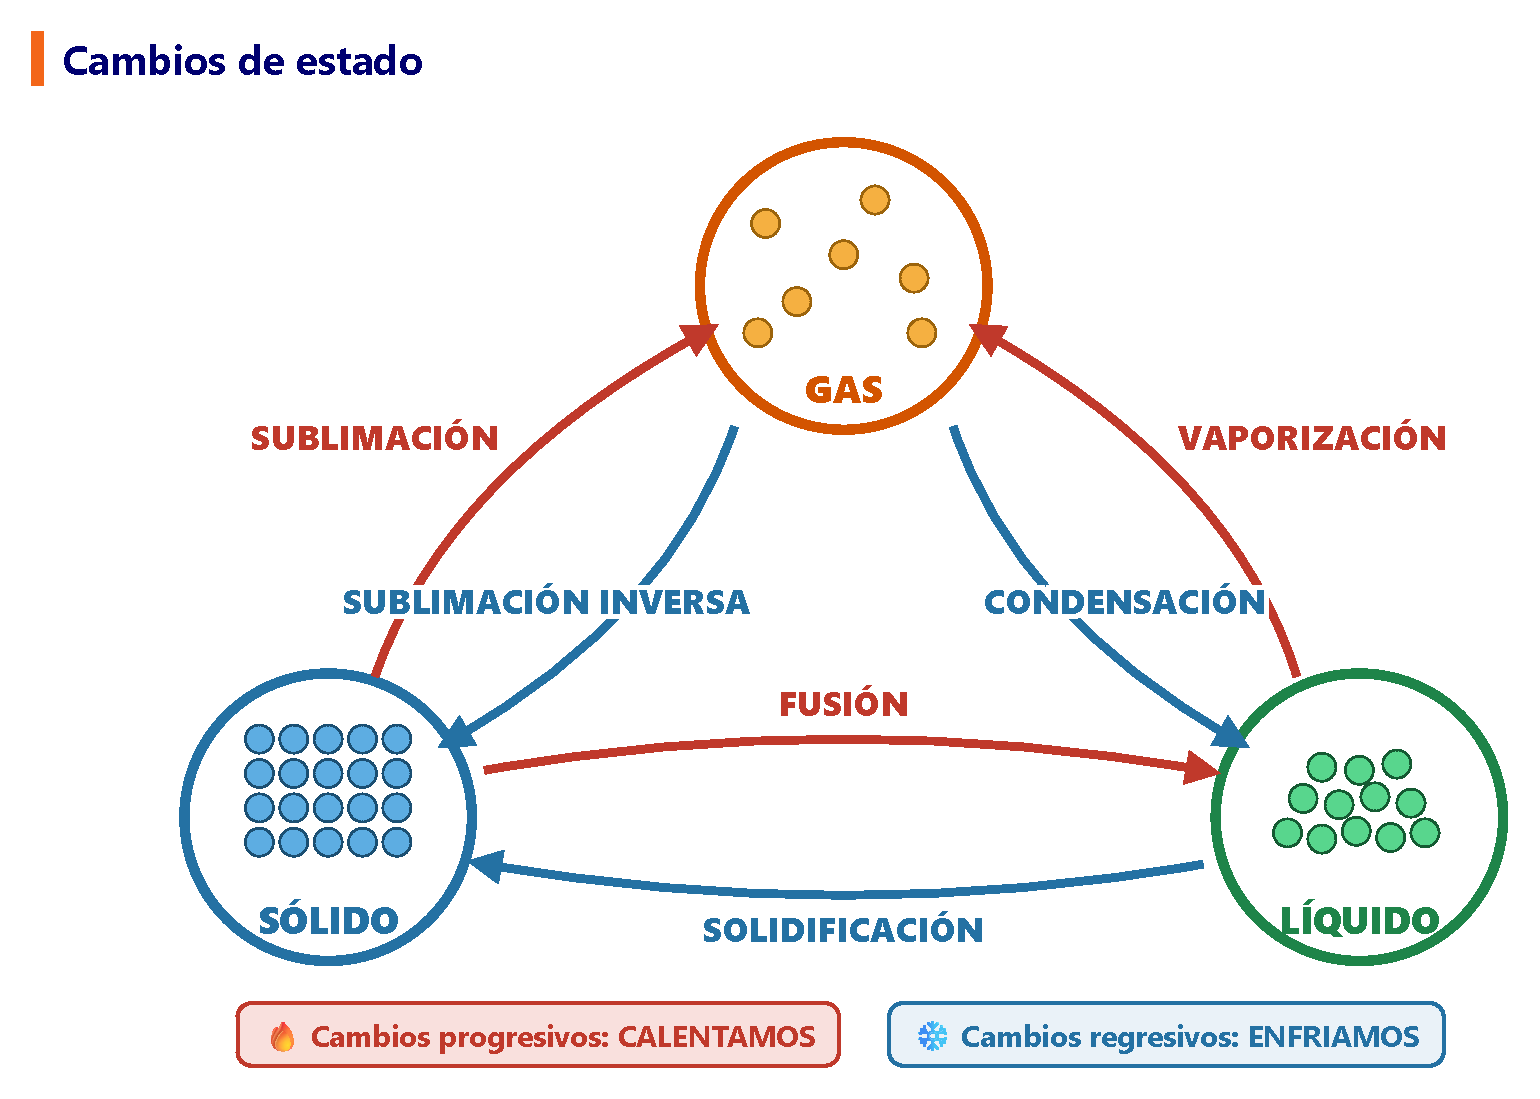
\includegraphics[width=0.95\textwidth]{FigurasSVG/Unit_2_State_of_Matter/pdf/changes_of_state_es.pdf}
    \caption{Los seis cambios de estado.}
    \label{fig:u2_changes_of_state}
\end{figure}

\begin{definition}[Punto de fusión y punto de ebullición]
    El \textbf{punto de fusión} es la temperatura a la que una sustancia pura pasa de sólido a líquido; el \textbf{punto de ebullición}, de líquido a gas. Los dos dependen de la presión y son \textbf{propiedades características}: cada sustancia tiene sus propios valores.
\end{definition}

\begin{table}[H]
    \centering
    \renewcommand{\arraystretch}{1.3}
    \begin{tabular}{lcc}
        \toprule
        \textbf{Sustancia} & \textbf{Punto de fusión} & \textbf{Punto de ebullición} \\
        \midrule
        Oxígeno & \qty{-219}{\celsius} & \qty{-183}{\celsius} \\
        Alcohol & \qty{-114}{\celsius} & \qty{78}{\celsius} \\
        Mercurio & \qty{-39}{\celsius} & \qty{357}{\celsius} \\
        Agua & \qty{0}{\celsius} & \qty{100}{\celsius} \\
        Hierro & \qty{1538}{\celsius} & \qty{2861}{\celsius} \\
        \bottomrule
    \end{tabular}
    \caption{Puntos de fusión y de ebullición de algunas sustancias.}
    \label{tab:u2_mp_bp}
\end{table}

\begin{impt}
    \textbf{¿En qué estado está a temperatura ambiente?} Por debajo de su punto de fusión, una sustancia es \textbf{sólida}; entre sus puntos de fusión y de ebullición es \textbf{líquida}; por encima de su punto de ebullición es un \textbf{gas}.
\end{impt}

\subsection{Curvas de calentamiento y calor latente}

Si calentamos hielo a ritmo constante y anotamos su temperatura cada minuto, obtenemos una \negsubro{curva de calentamiento}:

\begin{figure}[H]
    \centering
    % [FIGURA ORIGINAL] \includegraphics[width=\textwidth]{Unit_2/heating_curve}
    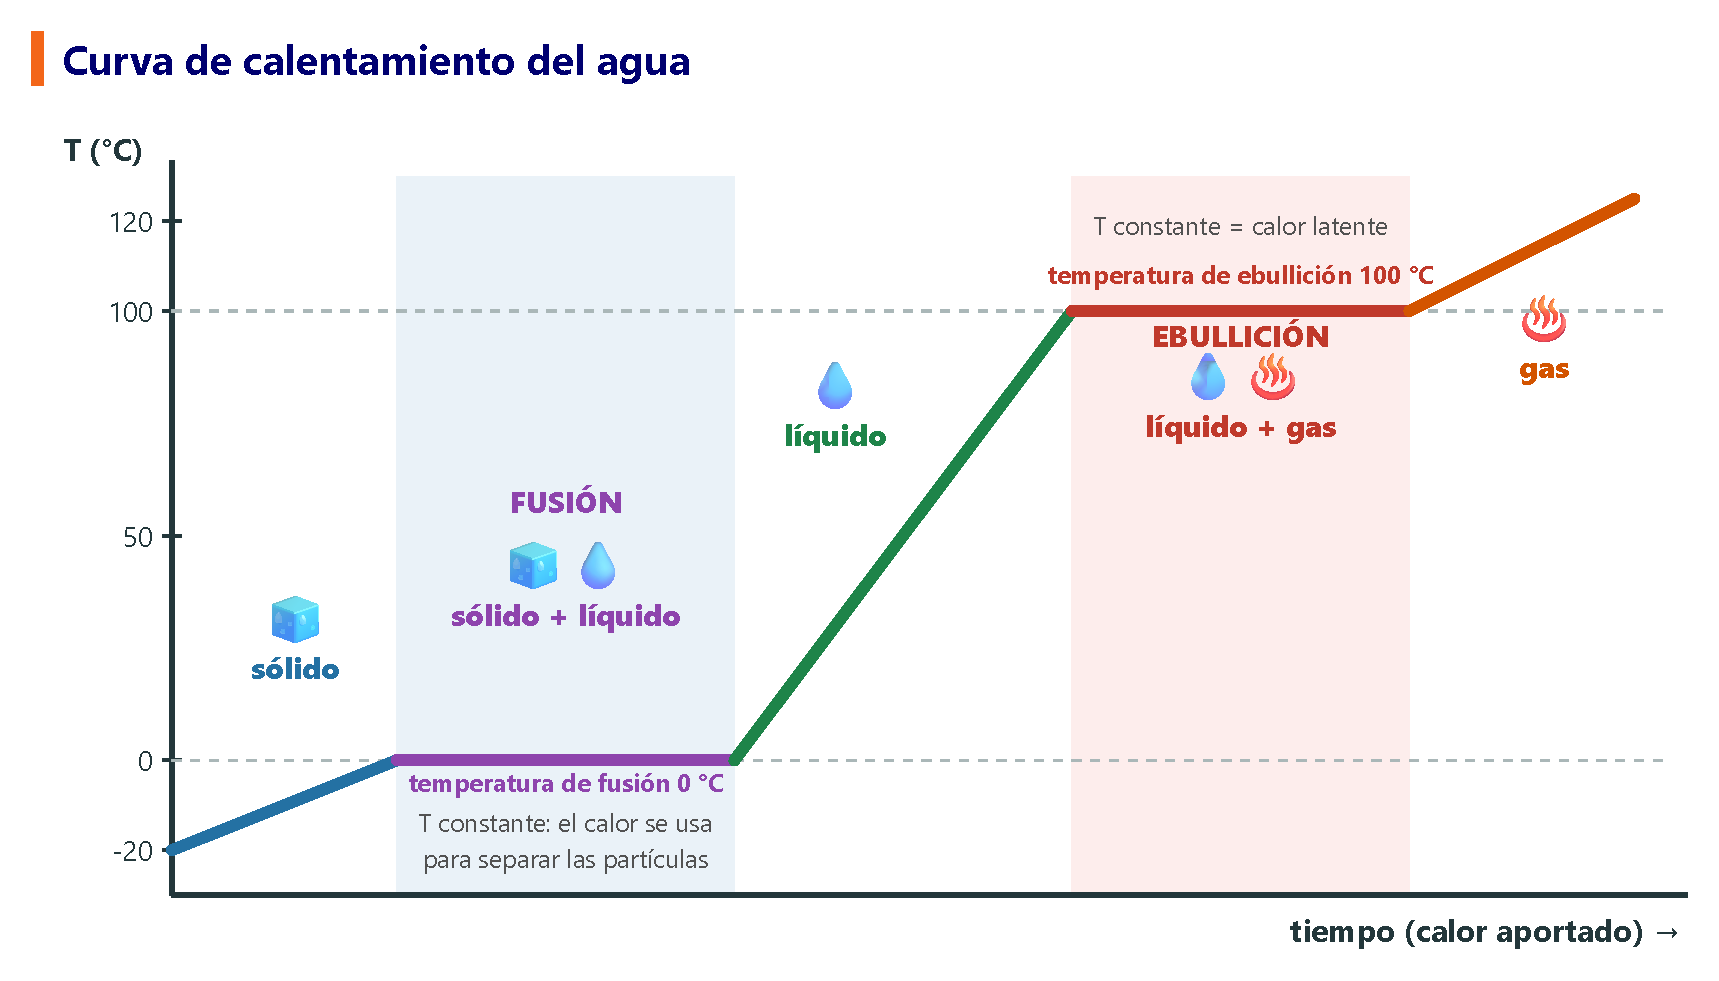
\includegraphics[width=\textwidth]{FigurasSVG/Unit_2_State_of_Matter/pdf/heating_curve_es.pdf}
    \caption{Curva de calentamiento del agua: la temperatura se mantiene constante durante cada cambio de estado.}
    \label{fig:u2_heating_curve}
\end{figure}

\begin{impt}
    Mientras una sustancia pura está \textbf{cambiando de estado}, su \textbf{temperatura no cambia}, aunque sigamos calentándola: la gráfica es horizontal (un «escalón» o meseta). Todo el calor se usa para separar las partículas, no para que se muevan más deprisa.
\end{impt}

\begin{definition}[Calor latente]
    Calor necesario para cambiar de estado \qty{1}{\kg} de una sustancia sin que cambie su temperatura. «Latente» significa «oculto»: damos calor, pero el termómetro no lo refleja.
\end{definition}

\subsection{Curvas de enfriamiento}

Si hacemos lo contrario y \textbf{enfriamos} una sustancia a ritmo constante mientras anotamos su temperatura cada minuto, obtenemos una \negsubro{curva de enfriamiento}. Parece la \textbf{imagen en un espejo} de la curva de calentamiento: la temperatura \textbf{baja}, y hay \textbf{mesetas} (tramos horizontales) a las \textbf{mismas temperaturas} que en la curva de calentamiento, mientras el gas se condensa y mientras el líquido se solidifica.

\begin{figure}[H]
    \centering
    % [FIGURA ORIGINAL] \includegraphics[width=\textwidth]{Unit_2/cooling_curve}
    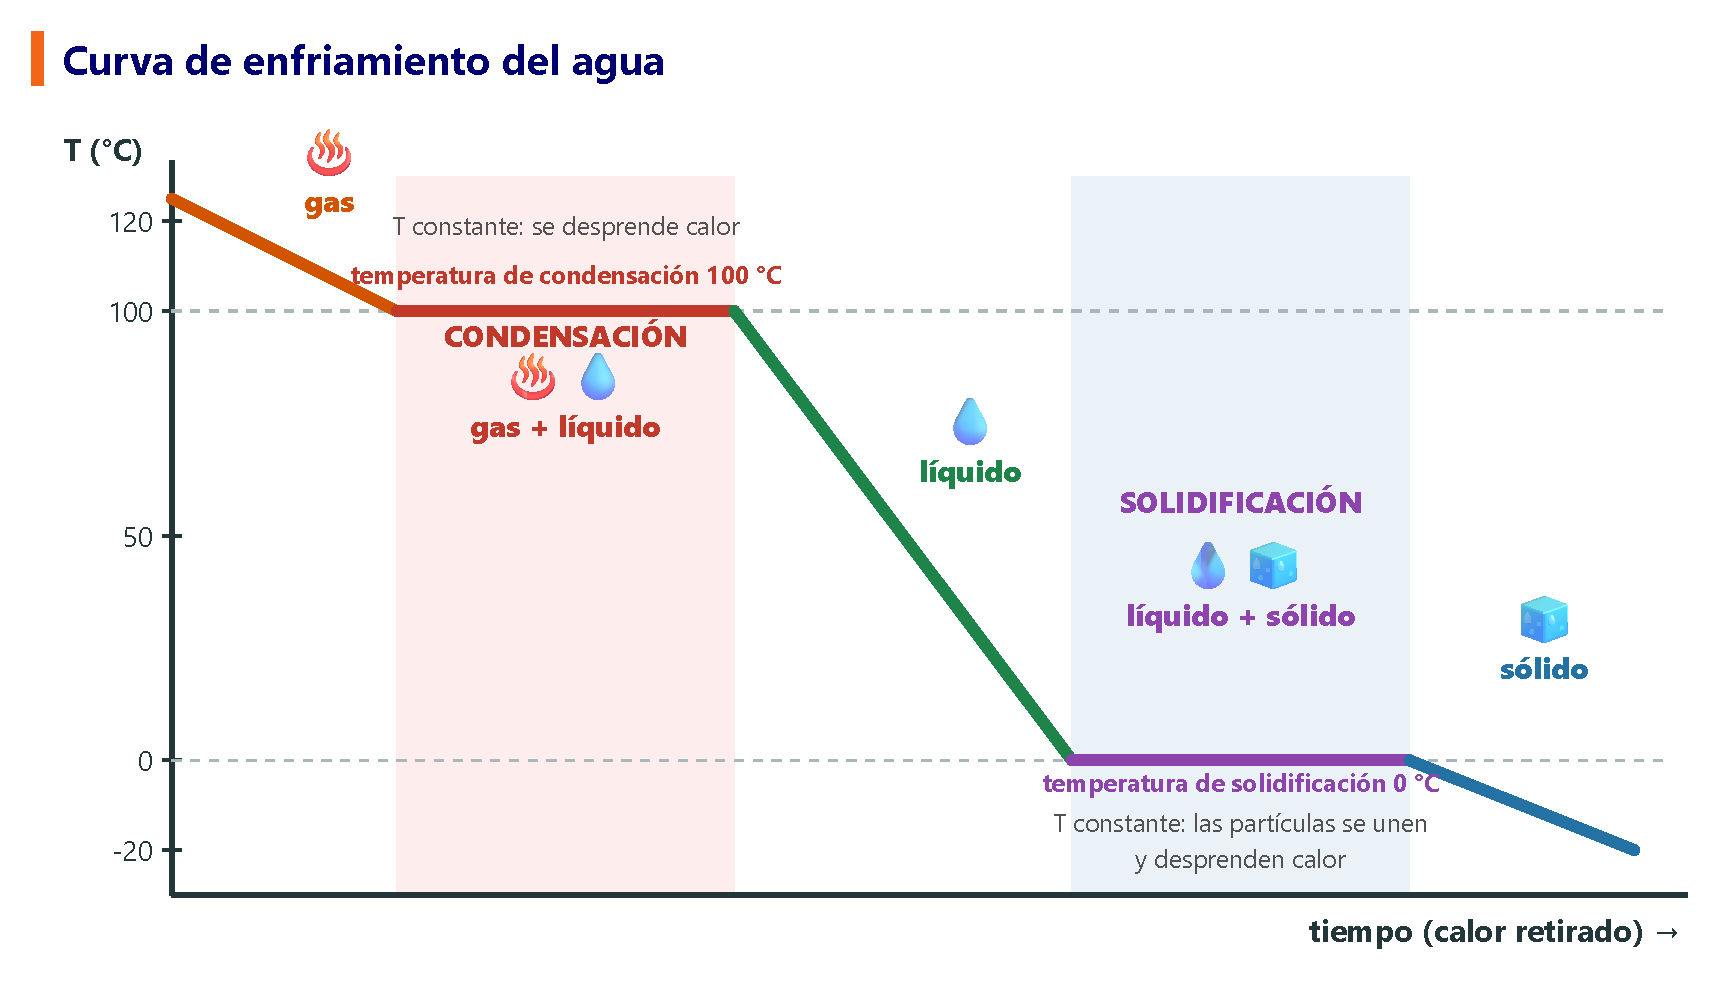
\includegraphics[width=\textwidth]{FigurasSVG/Unit_2_State_of_Matter/pdf/cooling_curve_es.pdf}
    \caption{Curva de enfriamiento del agua: la temperatura se mantiene constante mientras el vapor se condensa (\qty{100}{\celsius}) y mientras el líquido se solidifica (\qty{0}{\celsius}).}
    \label{fig:u2_cooling_curve}
\end{figure}

\begin{impt}
    \begin{itemize}
        \item En una curva de enfriamiento la sustancia \textbf{pierde} calor. En los tramos inclinados su temperatura baja; en los tramos horizontales está \textbf{cambiando de estado} (condensación o solidificación) y la temperatura \textbf{no} cambia.
        \item Una sustancia pura se \textbf{condensa} a la misma temperatura a la que \textbf{hierve}, y se \textbf{solidifica} a la misma temperatura a la que se \textbf{funde}. Para el agua: \qty{100}{\celsius} y \qty{0}{\celsius}.
    \end{itemize}
\end{impt}

\begin{example}
    \textbf{Lectura de la curva de enfriamiento del agua.} Partimos de vapor de agua a \qty{125}{\celsius} y le quitamos calor:
    \begin{enumerate}[label=\numberballmDarkTeal]
        \item De \qty{125}{\celsius} a \qty{100}{\celsius}: solo hay \textbf{gas}, y su temperatura baja.
        \item A \qty{100}{\celsius}: la línea es horizontal. El vapor se está \textbf{condensando}: hay \textbf{gas y líquido} a la vez y la temperatura no cambia.
        \item De \qty{100}{\celsius} a \qty{0}{\celsius}: solo hay \textbf{líquido}, y se va enfriando.
        \item A \qty{0}{\celsius}: la línea vuelve a ser horizontal. El agua se está \textbf{solidificando}: hay \textbf{líquido y sólido} a la vez.
        \item Por debajo de \qty{0}{\celsius}: solo hay \textbf{sólido} (hielo), y se sigue enfriando.
    \end{enumerate}
\end{example}

\begin{example}
    \textbf{Curva de enfriamiento de la parafina.} Se deja enfriar parafina líquida a \qty{80}{\celsius} y se anota su temperatura cada minuto:
    \begin{center}
        \renewcommand{\arraystretch}{1.3}
        % --- tabla antigua ---
        % \begin{tabular}{l|cccccccc}
            % \textbf{Time (min)} & 0 & 1 & 2 & 3 & 4 & 5 & 6 & 7 \\
            % \hline
            % \textbf{T (\unit{\celsius})} & 80 & 70 & 60 & 55 & 55 & 55 & 45 & 35 \\
        % \end{tabular}
        % --- tabla nueva ---
        \begin{tabular}{@{}lcccccccc@{}}
            \toprule
            \textbf{Tiempo (min)} & \textbf{0} & \textbf{1} & \textbf{2} & \textbf{3} & \textbf{4} & \textbf{5} & \textbf{6} & \textbf{7} \\
            \midrule
            \textbf{T (\unit{\celsius})} & 80 & 70 & 60 & 55 & 55 & 55 & 45 & 35 \\
            \bottomrule
        \end{tabular}
    \end{center}
    Del minuto 3 al minuto 5 la temperatura se mantiene en \qty{55}{\celsius}: esa es la meseta. Por tanto, la parafina se \textbf{solidifica} (y también se funde) a \textcolor{red}{\qty{55}{\celsius}}. Antes del minuto 3 la parafina es líquida, entre los minutos 3 y 5 hay parafina líquida y sólida a la vez, y después del minuto 5 es sólida.
\end{example}

\begin{example}
    \textbf{Ejemplo resuelto: lectura de una curva de calentamiento paso a paso.} En el laboratorio calentamos a ritmo constante una sustancia pura desconocida, empezando a \qty{-130}{\celsius}, y anotamos su temperatura cada minuto:
    \begin{center}
        \renewcommand{\arraystretch}{1.3}
        \begin{tabular}{@{}lcccccccccccc@{}}
            \toprule
            \textbf{Tiempo (min)} & \textbf{0} & \textbf{1} & \textbf{2} & \textbf{3} & \textbf{4} & \textbf{5} & \textbf{6} & \textbf{7} & \textbf{8} & \textbf{9} & \textbf{10} & \textbf{11} \\
            \midrule
            \textbf{T (\unit{\celsius})} & \(-130\) & \(-114\) & \(-114\) & \(-114\) & \(-50\) & 14 & 78 & 78 & 78 & 78 & 90 & 102 \\
            \bottomrule
        \end{tabular}
    \end{center}
    Queremos saber: \textbf{a)} su punto de fusión y su punto de ebullición; \textbf{b)} su estado físico en cada tramo del experimento; \textbf{c)} de qué sustancia se trata.
    \begin{enumerate}[label=\numberballmDarkTeal]
        \item \textbf{Dibuja la gráfica.} Pon el \textbf{tiempo} en el eje horizontal y la \textbf{temperatura} en el eje vertical, elige una escala en la que quepan todos los valores (de \qty{-140}{\celsius} a \qty{120}{\celsius}), representa cada pareja de valores con un punto y une los puntos con líneas rectas (Figura~\ref{fig:u2_heating_curve_example}).
        \item \textbf{Busca las mesetas.} Buscamos los tramos de la tabla en los que la temperatura \textbf{no cambia}, aunque sigamos calentando:
        \begin{itemize}
            \item del minuto 1 al minuto 3 la temperatura se mantiene en \qty{-114}{\celsius};
            \item del minuto 6 al minuto 9 la temperatura se mantiene en \qty{78}{\celsius}.
        \end{itemize}
        \item \textbf{Pon nombre a los cambios de estado.} Estamos \textbf{calentando}, así que la primera meseta (la de menor temperatura) es la \textbf{fusión} y la segunda (la de mayor temperatura) es la \textbf{ebullición}. Por tanto:
        \[
            \text{punto de fusión} = \textcolor{red}{\qty{-114}{\celsius}} \qquad \text{punto de ebullición} = \textcolor{red}{\qty{78}{\celsius}}
        \]
        \item \textbf{Escribe el estado en cada tramo.} Por debajo del punto de fusión la sustancia es sólida; en una meseta hay dos estados a la vez; entre las dos mesetas es líquida; por encima del punto de ebullición es gas:
        \begin{itemize}
            \item de 0 a 1 min: \textbf{sólido}, y su temperatura sube;
            \item de 1 a 3 min: \textbf{sólido + líquido} (se está fundiendo), temperatura constante;
            \item de 3 a 6 min: \textbf{líquido}, y su temperatura sube;
            \item de 6 a 9 min: \textbf{líquido + gas} (está hirviendo), temperatura constante;
            \item de 9 a 11 min: \textbf{gas}, y su temperatura sube.
        \end{itemize}
        \item \textbf{Identifica la sustancia.} Los puntos de fusión y de ebullición son \textbf{propiedades características}, así que comparamos nuestros valores con la Tabla~\ref{tab:u2_mp_bp}: la sustancia que funde a \qty{-114}{\celsius} y hierve a \qty{78}{\celsius} es el \textcolor{red}{\textbf{alcohol}}.
        \item \textbf{Comprueba la respuesta.} A temperatura ambiente (\qty{20}{\celsius}) nuestra sustancia estaría entre sus puntos de fusión y de ebullición, así que sería un \textbf{líquido}. Es correcto: el alcohol es líquido a temperatura ambiente.
    \end{enumerate}
\end{example}

\begin{figure}[H]
    \centering
    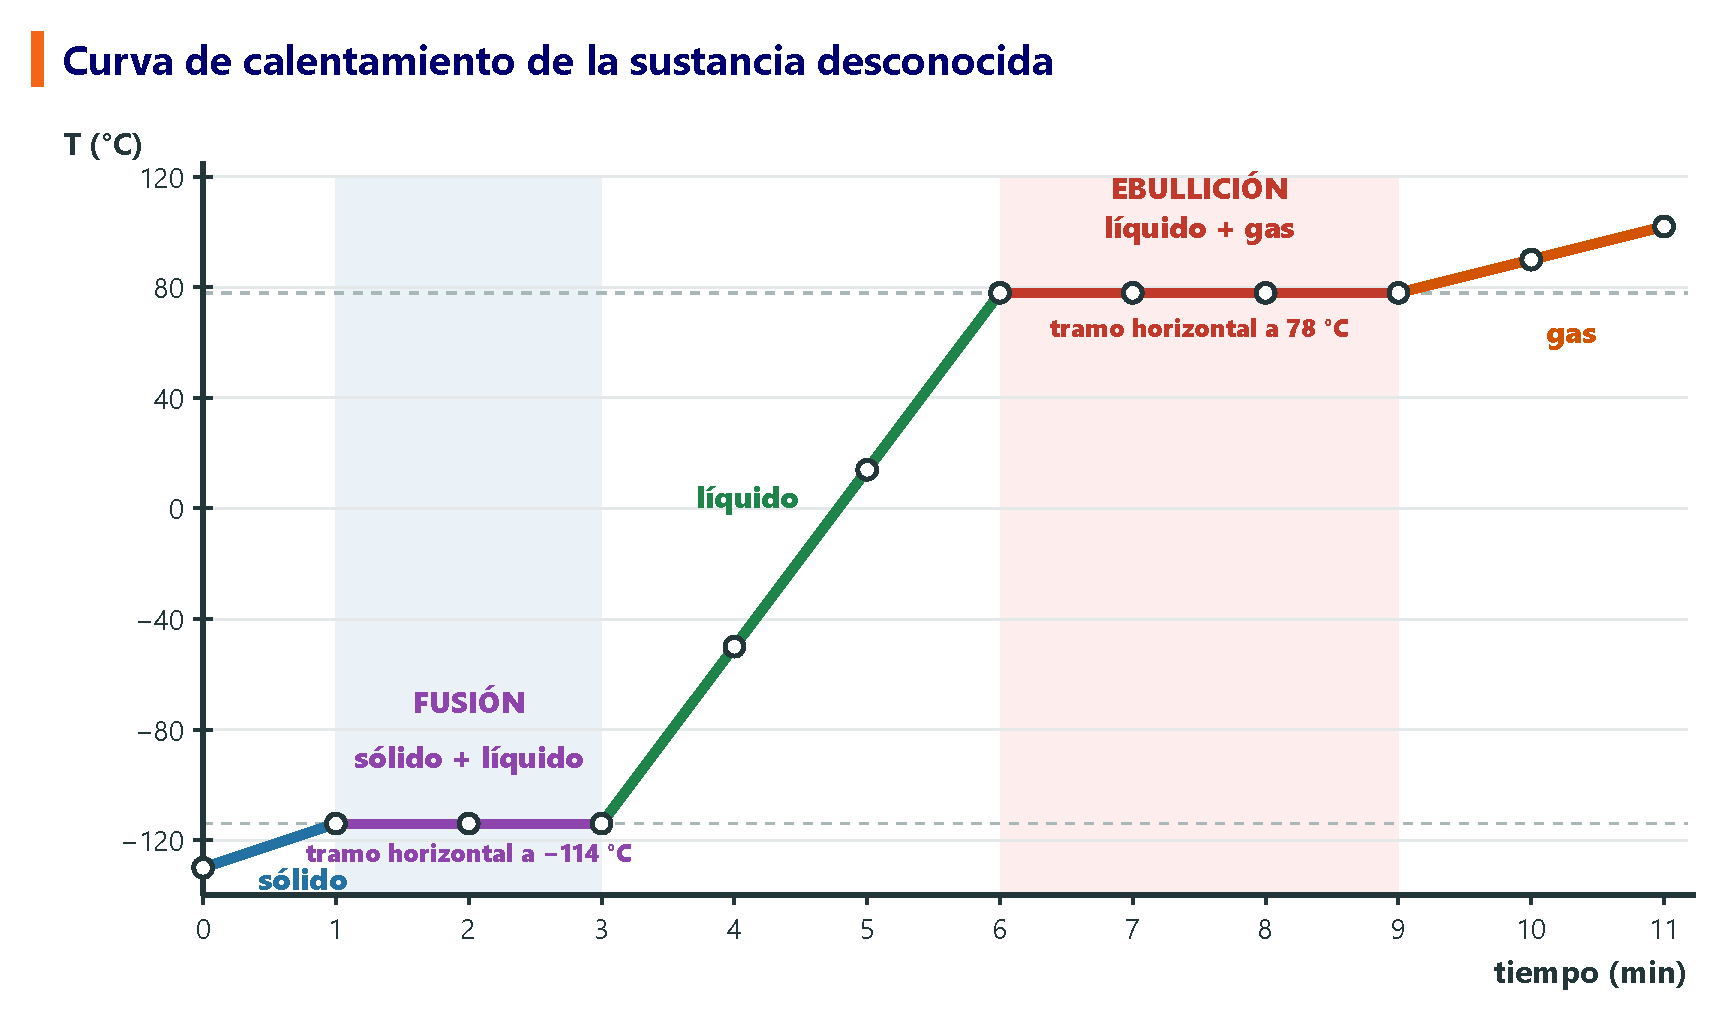
\includegraphics[width=\textwidth]{FigurasSVG/Unit_2_State_of_Matter/pdf/heating_curve_example_es.pdf}
    \caption{Curva de calentamiento dibujada con los datos del ejemplo resuelto: las mesetas a \qty{-114}{\celsius} y \qty{78}{\celsius} son los puntos de fusión y de ebullición del alcohol.}
    \label{fig:u2_heating_curve_example}
\end{figure}

\begin{exercise}
    Se calienta a ritmo constante una muestra de una sustancia pura y se anota su temperatura cada minuto: \qty{-10}{\celsius}, \qty{0}{\celsius}, \qty{0}{\celsius}, \qty{0}{\celsius}, \qty{20}{\celsius}, \qty{40}{\celsius} (en \(t = 0, 1, 2, 3, 4, 5\) min).
    \begin{enumerate}[label=\letraminuscula]
        \item ¿Cuál es el punto de fusión de la sustancia?
        \item ¿En qué minutos está cambiando de estado la sustancia? ¿Qué estados coexisten?
        \item ¿Podría ser agua esta sustancia? Justifica tu respuesta.
    \end{enumerate}
    \begin{solu}
        \begin{enumerate}[label=\alph*)]
            \item La temperatura se mantiene constante en \qty{0}{\celsius}, así que el punto de fusión es \qty{0}{\celsius}.
            \item Entre \(t = 1\) y \(t = 3\) min; coexisten \textbf{sólido y líquido}.
            \item \textbf{Sí}, podría ser agua: su punto de fusión (\qty{0}{\celsius}) coincide con el punto de fusión del agua a \qty{1}{\atmospher}.
        \end{enumerate}
    \end{solu}
\end{exercise}

\begin{exercise}
    Cera de vela fundida se enfría a temperatura ambiente, y se anota su temperatura cada 2 minutos: \qty{80}{\celsius}, \qty{60}{\celsius}, \qty{45}{\celsius}, \qty{45}{\celsius}, \qty{45}{\celsius}, \qty{45}{\celsius}, \qty{30}{\celsius}, \qty{22}{\celsius} (en \(t = 0, 2, 4, 6, 8, 10, 12, 14\) min).
    \begin{enumerate}[label=\letraminuscula]
        \item Dibuja la curva de enfriamiento (temperatura en el eje vertical, tiempo en el eje horizontal).
        \item ¿Cuál es el punto de solidificación de la cera?
        \item ¿Durante qué minutos está cambiando de estado la cera, y qué estados coexisten?
    \end{enumerate}
    \begin{solu}
        \begin{enumerate}[label=\alph*)]
            \item La curva baja de \qty{80}{\celsius} a \qty{45}{\celsius}, se mantiene horizontal en \qty{45}{\celsius} durante varios minutos y luego vuelve a bajar hasta \qty{22}{\celsius}.
            \item \qty{45}{\celsius}.
            \item Entre \(t = 4\) y \(t = 10\) min; coexisten cera \textbf{líquida y sólida}.
        \end{enumerate}
    \end{solu}
\end{exercise}

\begin{exercise}
    Un alumno dice: «Si pongo el fuego de la cocina al máximo, el agua de la olla hervirá a una temperatura mucho más alta, así que la pasta se hará antes». ¿Tiene razón? Utiliza la idea de calor latente.
    \begin{solu}
        El alumno \textbf{se equivoca}. Cuando el agua llega a su punto de ebullición (\qty{100}{\celsius} a \qty{1}{\atmospher}), su temperatura se mantiene constante por mucho calor que le demos. Más calor solo hace que el agua hierva \textbf{con más fuerza}: el calor extra se usa como calor latente para convertir más líquido en gas, no para subir la temperatura.
    \end{solu}
\end{exercise}

\subsection{Evaporación y ebullición}

\begin{figure}[H]
    \centering
    % [FIGURA ORIGINAL] \includegraphics[width=\textwidth]{Unit_2/evaporation_boiling}
    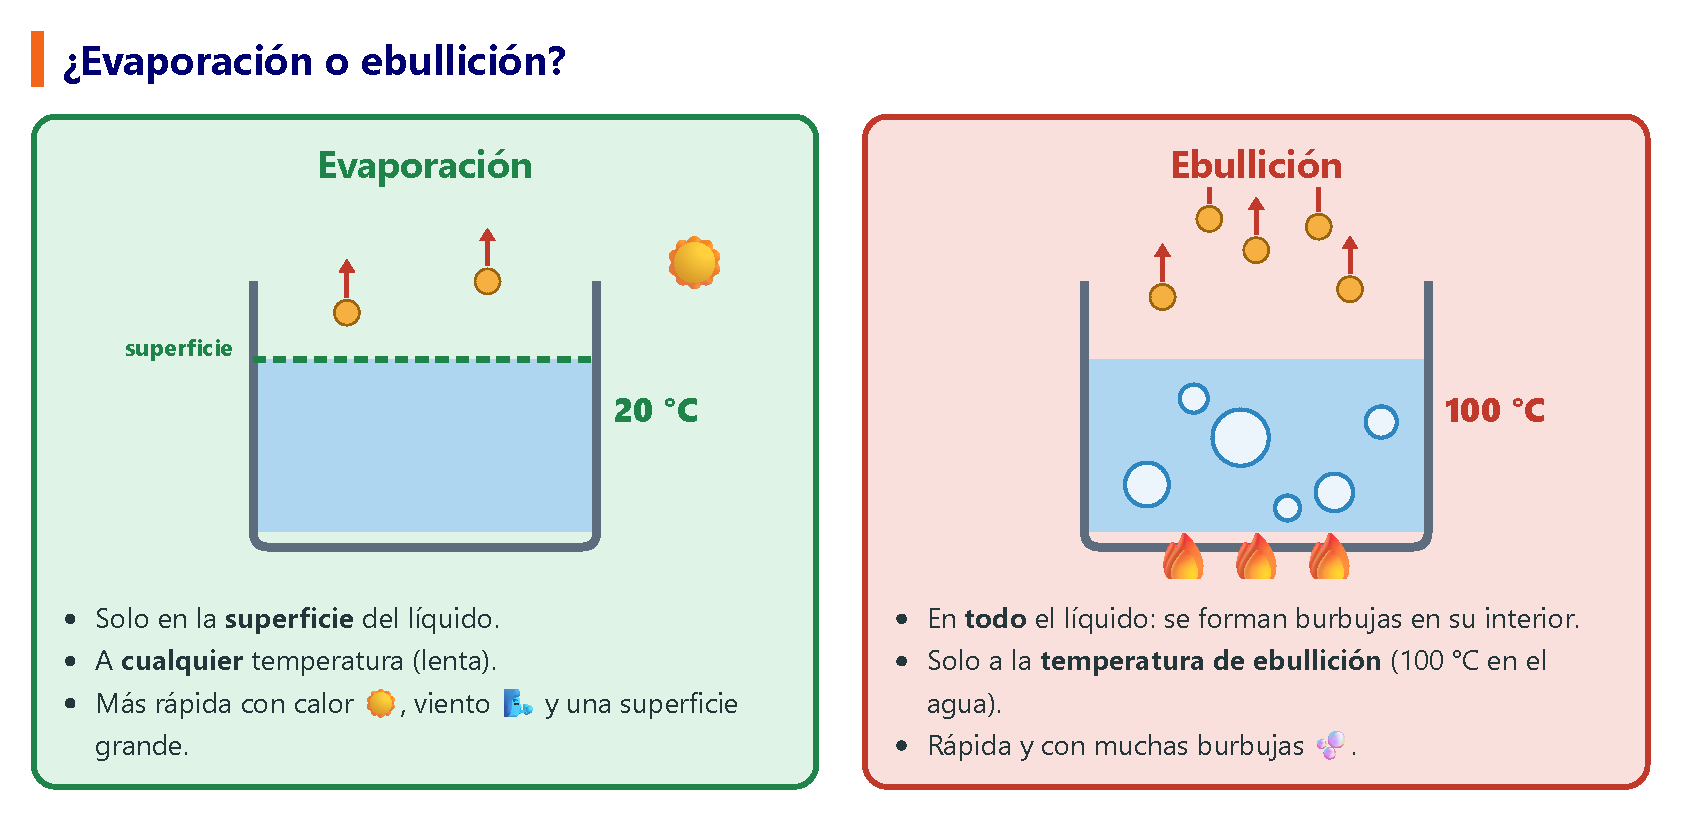
\includegraphics[width=\textwidth]{FigurasSVG/Unit_2_State_of_Matter/pdf/evaporation_boiling_es.pdf}
    \caption{Dos formas de convertir un líquido en gas.}
    \label{fig:u2_evaporation_boiling}
\end{figure}

\begin{exercise}
    Clasifica cada situación como evaporación o ebullición, y justifica tu respuesta.
    \begin{enumerate}[label=\letraminuscula]
        \item La ropa mojada tendida en el tendedero se seca al cabo de unas horas.
        \item El agua de un cazo burbujea con fuerza en el fuego a \qty{100}{\celsius}.
        \item Un charco de la acera desaparece poco a poco durante una tarde templada.
        \item La leche de un cazo sube y burbujea por todas partes justo antes de «salirse».
    \end{enumerate}
    \begin{solu}
        \begin{enumerate}[label=\alph*)]
            \item \textbf{Evaporación}: en la superficie de la tela mojada, muy por debajo de \qty{100}{\celsius}.
            \item \textbf{Ebullición}: se forman burbujas en todo el líquido, a su punto de ebullición.
            \item \textbf{Evaporación}: solo en la superficie del charco, a la temperatura del exterior.
            \item \textbf{Ebullición}: afecta a toda la masa de leche, no solo a la superficie.
        \end{enumerate}
    \end{solu}
\end{exercise}

\begin{exercise}
    Explica por qué la ropa tendida se seca antes en un día soleado y con viento que en un día nublado y sin viento, y por qué también se seca antes si la extendemos bien.
    \begin{solu}
        El secado de la ropa es una \textbf{evaporación}. El Sol aumenta la temperatura, así que las partículas de agua tienen más energía para escapar; el viento se lleva el vapor en cuanto se forma. Al extender la ropa aumentamos la \textbf{superficie}, y la evaporación es más rápida cuanto mayor es la superficie.
    \end{solu}
\end{exercise}

\subsection{Sublimación y sublimación inversa}

Algunas sustancias, como el yodo o el dióxido de carbono sólido («hielo seco»), pasan directamente de sólido a gas, o de gas a sólido, \textbf{sin} pasar por líquido:

\begin{itemize}
    \item \negsubro{Sublimación}: sólido \(\to\) gas.
    \item \negsubro{Sublimación inversa} (o regresiva): gas \(\to\) sólido (por ejemplo, la escarcha de una mañana fría).
\end{itemize}

\begin{impt}
    Los cambios que se producen al \textbf{calentar} (fusión, evaporación, sublimación) son \negsubro{progresivos}. Los cambios que se producen al \textbf{enfriar} (solidificación, condensación, sublimación inversa) son \negsubro{regresivos}.
\end{impt}

\begin{didyouknow}
    ¡El «humo» que sale del hielo seco en los conciertos no es dióxido de carbono gaseoso, que es invisible! El gas, muy frío, enfría el aire que lo rodea, y el vapor de agua del aire se condensa en gotitas diminutas: una niebla artificial.
\end{didyouknow}

\begin{exercise}
    En los escenarios se suelen usar bloques de dióxido de carbono sólido («hielo seco») para crear un efecto de niebla.
    \begin{enumerate}[label=\letraminuscula]
        \item ¿Qué cambio de estado se produce cuando el hielo seco «desaparece»? ¿Es progresivo o regresivo?
        \item A diferencia de un cubito de hielo, el hielo seco nunca deja un charco de líquido. ¿Por qué?
    \end{enumerate}
    \begin{solu}
        \begin{enumerate}[label=\alph*)]
            \item \textbf{Sublimación} (sólido \(\to\) gas), un cambio \textbf{progresivo}.
            \item A presión atmosférica, el dióxido de carbono sólido pasa directamente de sólido a gas, sin pasar por el estado líquido.
        \end{enumerate}
    \end{solu}
\end{exercise}

\begin{exercise}
    Las bolas de naftalina (antipolillas) se van haciendo más pequeñas con las semanas, aunque nunca se calientan, y al final desaparecen sin dejar ningún líquido. Explica qué está ocurriendo y nombra el cambio de estado.
    \begin{solu}
        La bola de naftalina se está \textbf{sublimando}: sus partículas pasan directamente de sólido a gas (desprendiendo un olor que ahuyenta a los insectos), sin llegar a ser líquido. Esto puede ocurrir lentamente a temperatura ambiente.
    \end{solu}
\end{exercise}

\subsection{Efecto de la presión en la ebullición}

\begin{figure}[H]
    \centering
    % [FIGURA ORIGINAL] \includegraphics[width=\textwidth]{Unit_2/pressure_boiling}
    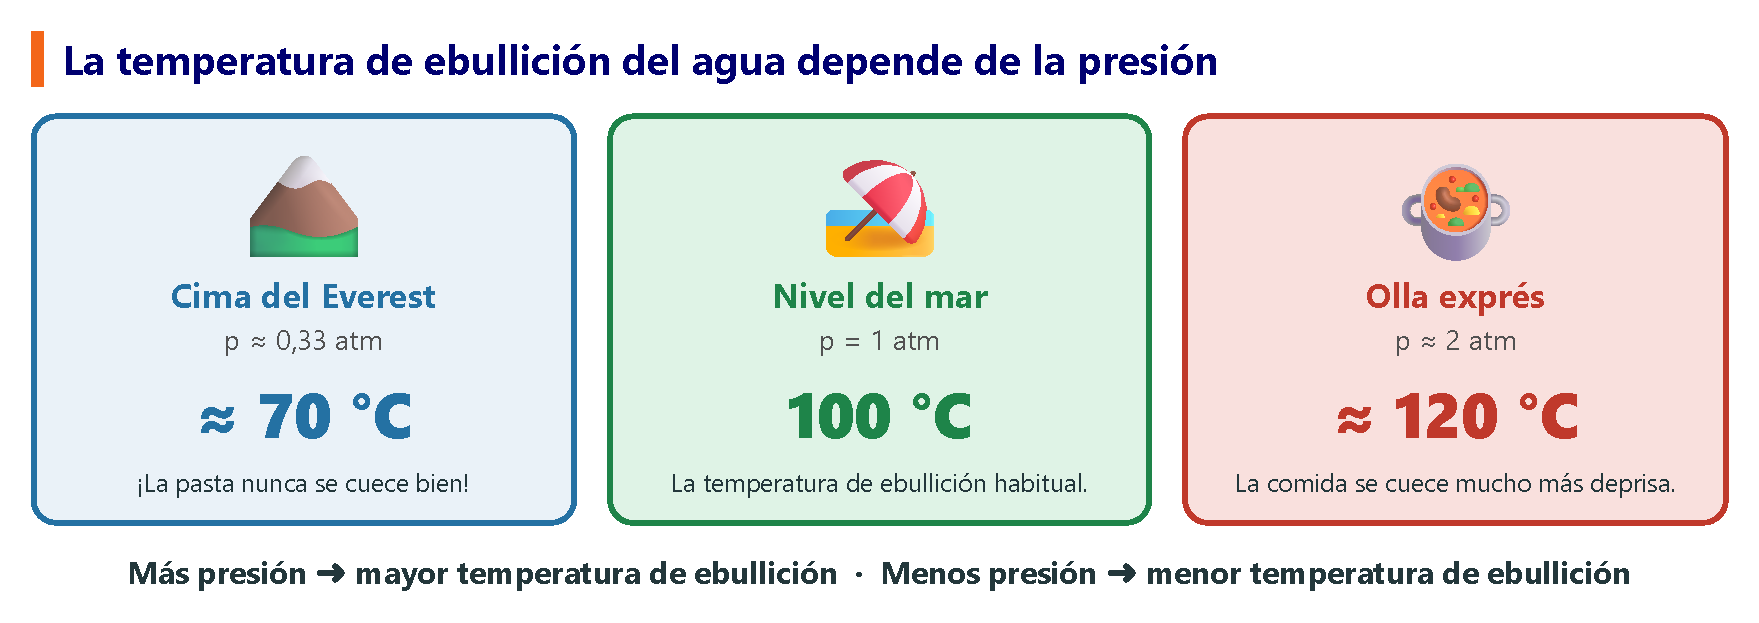
\includegraphics[width=\textwidth]{FigurasSVG/Unit_2_State_of_Matter/pdf/pressure_boiling_es.pdf}
    \caption{El punto de ebullición del agua cambia con la presión.}
    \label{fig:u2_pressure_boiling}
\end{figure}

\begin{exercise}
    Utiliza la tabla de puntos de fusión y de ebullición del principio de este apartado para indicar el estado físico del oxígeno, el alcohol, el agua y el hierro a \qty{20}{\celsius} y \qty{1}{\atmospher}.
    \begin{solu}
        Oxígeno: \textbf{gas} (\(20 > -183\)). \\
        Alcohol: \textbf{líquido} (\(-114 < 20 < 78\)). \\
        Agua: \textbf{líquido} (\(0 < 20 < 100\)). \\
        Hierro: \textbf{sólido} (\(20 < 1538\)).
    \end{solu}
\end{exercise}

\begin{exercise}
    Un líquido se enfría en un congelador. Su temperatura se anota cada \qty{10}{\minute}: \qty{20}{\celsius}, \qty{6}{\celsius}, \qty{-8}{\celsius}, \qty{-8}{\celsius}, \qty{-8}{\celsius}, \qty{-22}{\celsius} (en \(t = 0, 10, 20, 30, 40, 50\) min).
    \begin{enumerate}[label=\letraminuscula]
        \item ¿Cuál es el punto de solidificación de esta sustancia?
        \item ¿Puede ser agua esta sustancia? ¿Por qué?
    \end{enumerate}
    \begin{solu}
        \begin{enumerate}[label=\alph*)]
            \item La temperatura se mantiene constante en \qty{-8}{\celsius} entre \(t = 20\) y \(t = 40\) min, así que el punto de solidificación es \qty{-8}{\celsius}.
            \item \textbf{No}, porque el agua se solidifica a \qty{0}{\celsius}.
        \end{enumerate}
    \end{solu}
\end{exercise}

\begin{exercise}
    Un charco se seca en un día soleado; el espejo del baño se empaña durante una ducha caliente; se forma escarcha en las hojas en una noche muy fría y despejada; un polo gotea al sol. Identifica el cambio de estado en cada caso y di si es progresivo o regresivo.
    \begin{solu}
        Charco: \textbf{evaporación}, progresivo. \\
        Espejo: \textbf{condensación}, regresivo. \\
        Escarcha: \textbf{sublimación inversa}, regresivo. \\
        Polo: \textbf{fusión}, progresivo.
    \end{solu}
\end{exercise}

%----------------------------------------------------------------------------------------

\section{Estados del agua y meteorología}

El agua es la única sustancia que encontramos de forma natural en los tres estados en la Tierra. Sus cambios de estado producen el tiempo atmosférico que vemos cada día:

\begin{figure}[H]
    \centering
    % [FIGURA ORIGINAL] \includegraphics[width=\textwidth]{Unit_2/weather_phenomena}
    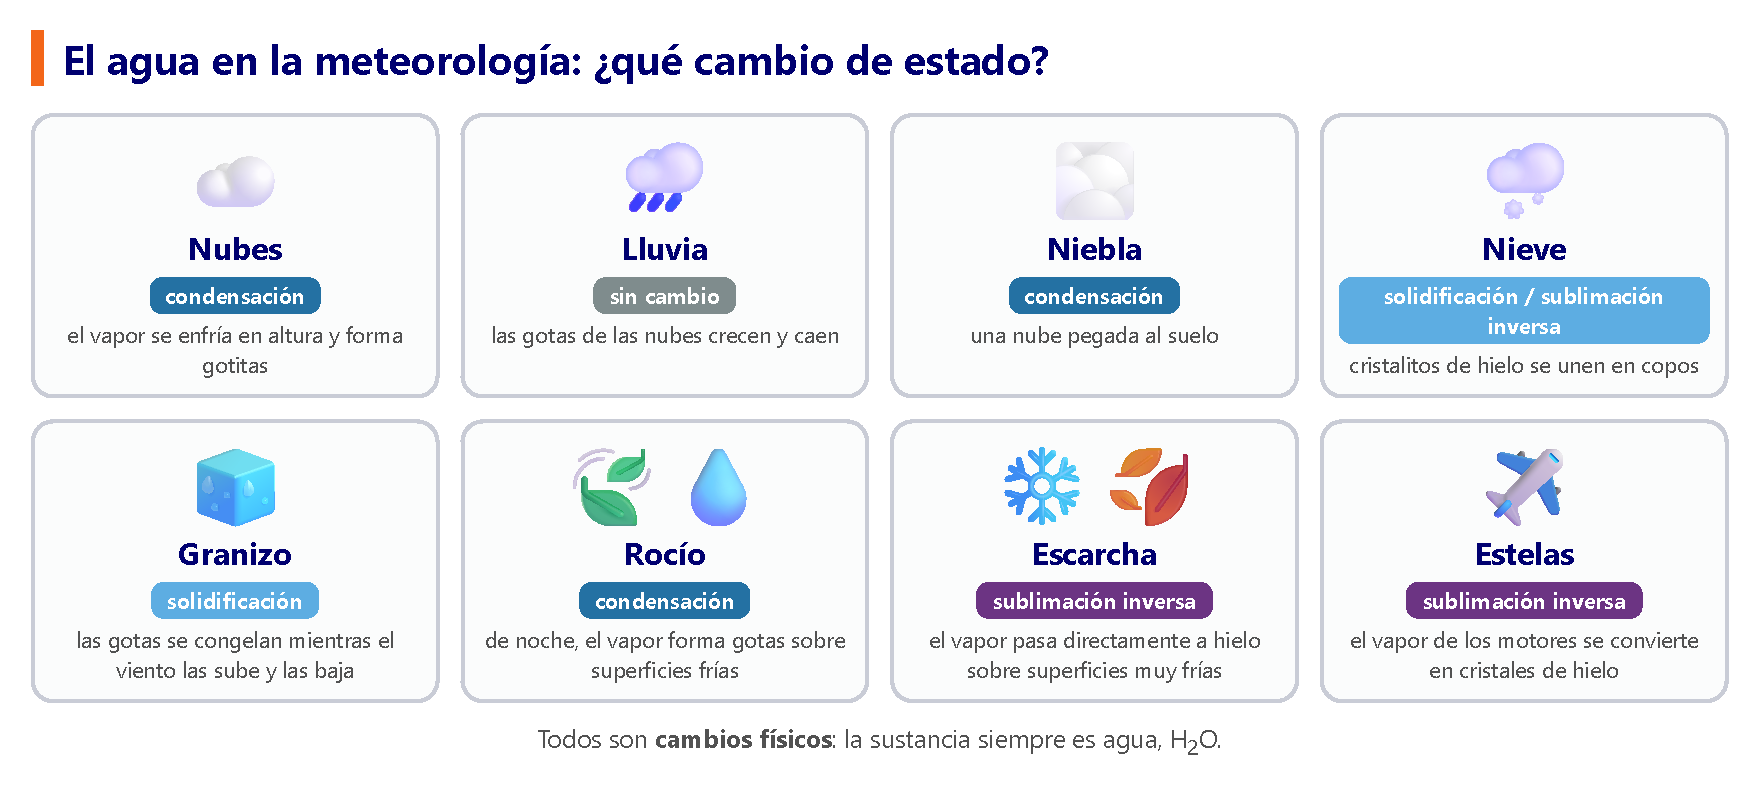
\includegraphics[width=\textwidth]{FigurasSVG/Unit_2_State_of_Matter/pdf/weather_phenomena_es.pdf}
    \caption{Fenómenos meteorológicos y el cambio de estado que hay detrás de cada uno.}
    \label{fig:u2_weather_phenomena}
\end{figure}

\begin{exercise}
    Indica en qué estado físico se encuentra el agua en: las nubes, el aire, el granizo, la nieve, el rocío, la escarcha.
    \begin{solu}
        Nubes: líquido (gotas) o sólido (cristales de hielo). Aire: gas (vapor de agua). Granizo: sólido. Nieve: sólido. Rocío: líquido. Escarcha: sólido.
    \end{solu}
\end{exercise}

\begin{exercise}
    Cuando respiramos en un día frío de invierno, vemos salir una pequeña nube de nuestra boca, pero dentro de casa no ocurre. ¿Por qué?
    \begin{solu}
        Nuestro aliento contiene vapor de agua caliente. En la calle, con el aire frío, se enfría muy deprisa y se \textbf{condensa} en gotitas diminutas que se ven. Dentro de casa el aire está más caliente, así que el vapor no se condensa y sigue siendo un gas invisible.
    \end{solu}
\end{exercise}

\begin{exercise}
    Relaciona cada fenómeno meteorológico con el cambio de estado que interviene, y di si es progresivo o regresivo: (1) rocío, (2) escarcha, (3) niebla, (4) granizo.
    \begin{enumerate}[label=\letraminuscula]
        \item[A] Condensación del vapor de agua en gotas de líquido.
        \item[B] Sublimación inversa del vapor de agua, que pasa directamente a sólido.
        \item[C] Evaporación seguida de condensación cerca del suelo.
        \item[D] Solidificación de gotas de líquido que suben y bajan dentro de una nube.
    \end{enumerate}
    \begin{solu}
        (1) Rocío \(\to\) A, condensación, regresivo. \\
        (2) Escarcha \(\to\) B, sublimación inversa, regresivo. \\
        (3) Niebla \(\to\) C, evaporación (progresivo) seguida de condensación (regresivo); la niebla que vemos se forma por condensación. \\
        (4) Granizo \(\to\) D, solidificación, regresivo.
    \end{solu}
\end{exercise}

\subsection{El ciclo del agua}

El agua se mueve continuamente entre el mar, el aire y la tierra, y cambia de estado por el camino. Es el \negsubro{ciclo del agua}, y su motor es el \textbf{Sol}.

\begin{figure}[H]
    \centering
    % [FIGURA ORIGINAL] \includegraphics[width=\textwidth]{Unit_2/water_cycle}
    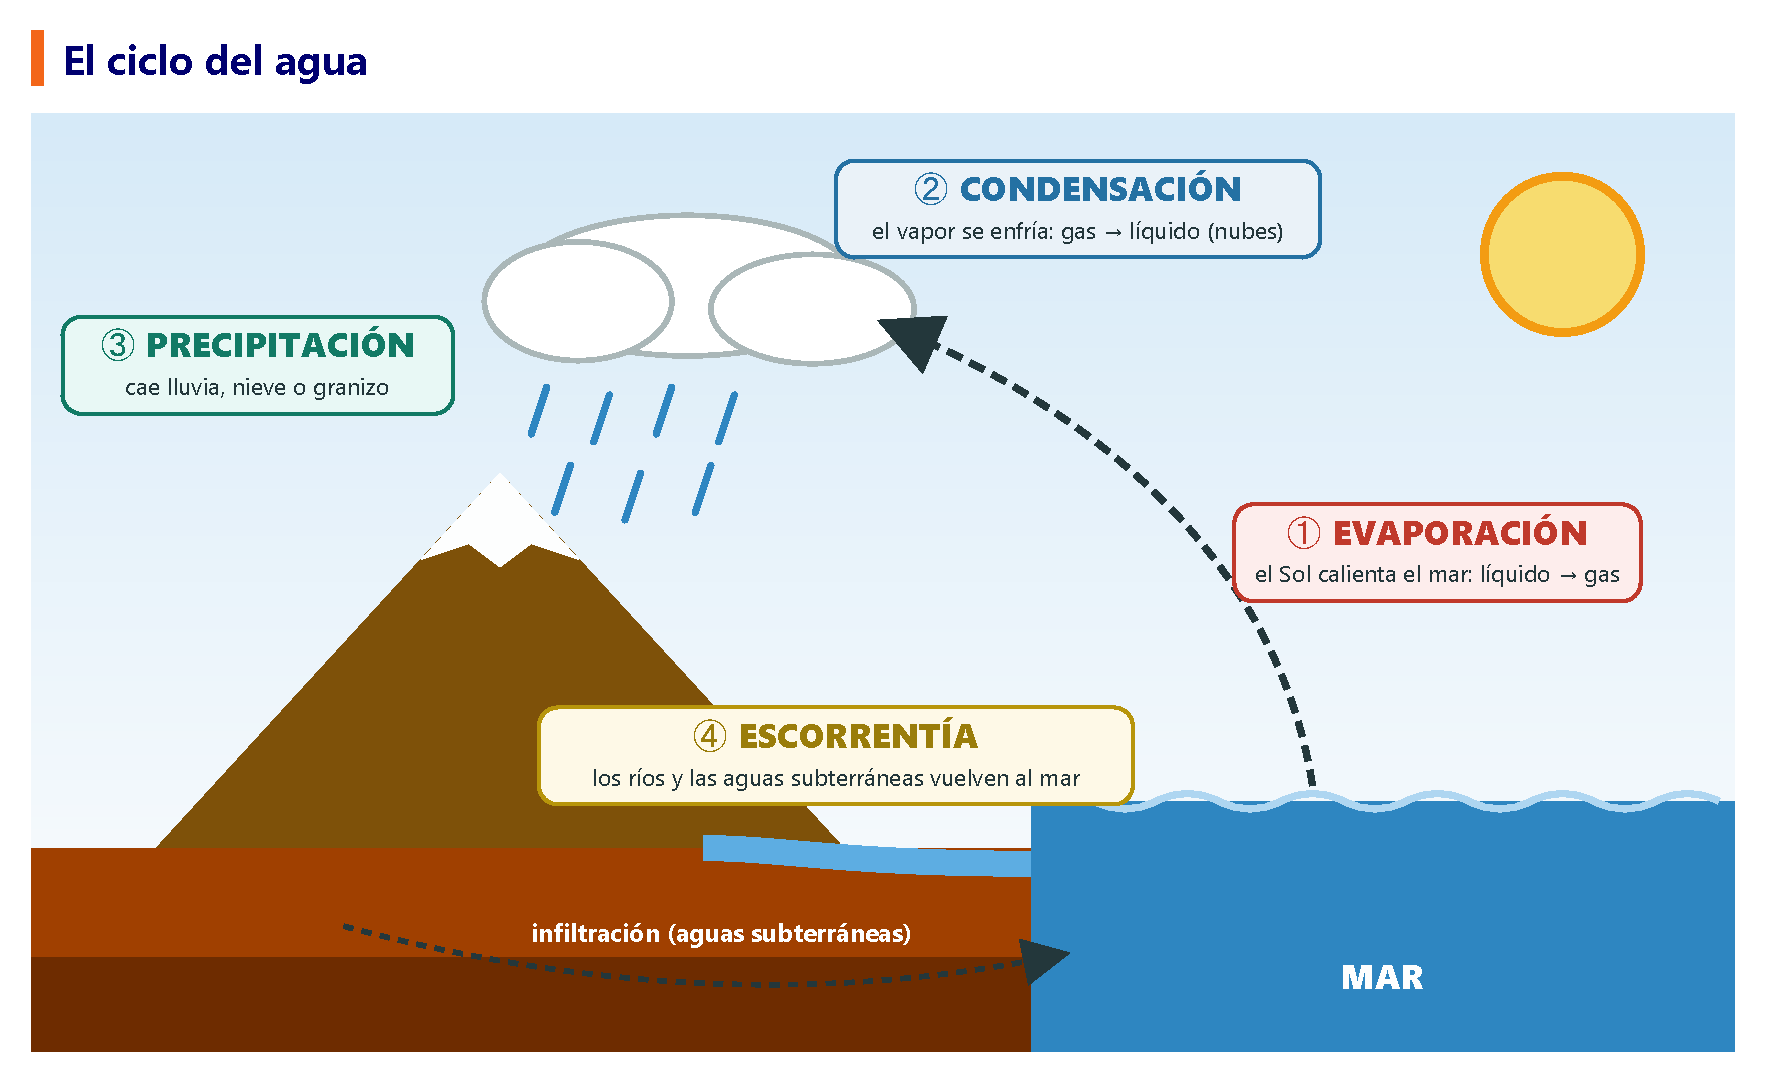
\includegraphics[width=\textwidth]{FigurasSVG/Unit_2_State_of_Matter/pdf/water_cycle_es.pdf}
    \caption{Las cuatro etapas del ciclo del agua.}
    \label{fig:u2_water_cycle}
\end{figure}

\begin{impt}
    En el ciclo del agua solo hay \textbf{cambios físicos}: la sustancia es siempre agua, \ch{H2O}, esté en el estado que esté.
\end{impt}

\begin{didyouknow}
    ¡El agua que bebes hoy es la misma que bebían los dinosaurios hace millones de años! La cantidad de agua de la Tierra apenas cambia: simplemente sigue dando vueltas y vueltas en el ciclo del agua.
\end{didyouknow}

\begin{exercise}
    Ordena correctamente estas etapas del ciclo del agua y nombra el cambio de estado que interviene en cada una: (1) se forman nubes sobre el mar; (2) llueve sobre las montañas; (3) el Sol calienta la superficie del océano; (4) los ríos devuelven el agua al mar.
    \begin{solu}
        Orden correcto: 3, 1, 2, 4. \\
        (3) El agua se convierte en vapor: \textbf{evaporación}. \\
        (1) El vapor de agua se enfría y forma gotitas diminutas: \textbf{condensación}. \\
        (2) Las gotitas crecen y caen: \textbf{precipitación} (no hay cambio de estado). \\
        (4) El agua líquida vuelve al mar (no hay cambio de estado).
    \end{solu}
\end{exercise}

\begin{exercise}
    Explica por qué se dice que en el ciclo del agua «solo hay cambios físicos», y por qué no podría continuar sin el Sol.
    \begin{solu}
        Aunque el agua cambia de estado muchas veces, siempre es la \textbf{misma sustancia}, \ch{H2O}: no se forman sustancias nuevas. El Sol aporta la energía necesaria para la \textbf{evaporación}; sin él no se formaría vapor de agua, no habría nubes ni precipitaciones.
    \end{solu}
\end{exercise}

\begin{exercise}
    «La mayor parte del agua que cae como lluvia sobre una cordillera se evaporó en el océano, a veces a cientos de kilómetros de distancia.»
    \begin{enumerate}[label=\letraminuscula]
        \item Describe, paso a paso, cómo una partícula de agua podría viajar desde el océano hasta una gota de lluvia que cae en una montaña.
        \item Una vez que la lluvia cae en la montaña, nombra dos caminos que puede seguir el agua.
    \end{enumerate}
    \begin{solu}
        \begin{enumerate}[label=\alph*)]
            \item El Sol calienta el océano y el agua se \textbf{evapora}. Los vientos llevan el vapor hacia el interior; al subir por las montañas se enfría y se \textbf{condensa} en gotitas diminutas (una nube). Cuando las gotitas son lo bastante grandes, caen en forma de \textbf{lluvia}.
            \item Puede correr por la superficie (arroyos y ríos) de vuelta al mar, o \textbf{infiltrarse} en el suelo y convertirse en agua subterránea.
        \end{enumerate}
    \end{solu}
\end{exercise}

%----------------------------------------------------------------------------------------

\section*{Resumen}

\begin{itemize}
    \item \textbf{Estados de la materia}: sólidos (forma y volumen fijos), líquidos (volumen fijo, forma variable), gases (forma y volumen variables).
    \item \textbf{Teoría cinética}: la materia está formada por partículas que están siempre en movimiento; cuanto más deprisa se mueven, mayor es la temperatura. Explica la difusión, la compresibilidad, la dilatación y la presión de los gases.
    \item \textbf{Presión de un gas}: se debe a los choques de las partículas del gas contra las paredes del recipiente.
    \item \textbf{Leyes de los gases} (temperatura siempre en kelvin, \(T(\unit{\K}) = T(\unit{\celsius}) + 273\)): Boyle-Mariotte (\(p \cdot V = \text{cte.}\)); Gay-Lussac (\(p/T = \text{cte.}\)); Charles (\(V/T = \text{cte.}\)); ley general de los gases (\(p \cdot V / T = \text{cte.}\)).
    \item \textbf{Cambios de estado}: progresivos (fusión, evaporación/ebullición, sublimación) y regresivos (solidificación, condensación, sublimación inversa). La temperatura se mantiene constante durante un cambio de estado, porque el calor se usa como \textbf{calor latente}.
    \item La \textbf{evaporación} se produce en la superficie, a cualquier temperatura; la \textbf{ebullición} se produce en todo el líquido, a la temperatura de ebullición.
    \item \textbf{Presión y punto de ebullición}: más presión \(\to\) punto de ebullición más alto (olla a presión); menos presión \(\to\) punto de ebullición más bajo (montaña).
    \item \textbf{Meteorología y ciclo del agua}: las nubes, la niebla y el rocío se forman por condensación; la escarcha y las estelas de los aviones, por sublimación inversa; el granizo, por solidificación. El Sol mueve el ciclo del agua: evaporación, condensación, precipitación y recogida.
\end{itemize}

\section{Vocabulario}

\begin{vocabulary}[Teoría cinética (\textit{kinetic theory})]
    Teoría que explica que la materia está formada por partículas en movimiento, cuyo comportamiento depende del estado en que se encuentre.
\end{vocabulary}

\begin{vocabulary}[Fusión (\textit{melting})]
    Cambio de estado de sólido a líquido.
\end{vocabulary}

\begin{vocabulary}[Solidificación (\textit{freezing})]
    Cambio de estado de líquido a sólido.
\end{vocabulary}

\begin{vocabulary}[Evaporación (\textit{evaporation})]
    Cambio de estado de líquido a gas que se produce en la superficie del líquido.
\end{vocabulary}

\begin{vocabulary}[Ebullición (\textit{boiling})]
    Cambio de estado de líquido a gas que se produce en todo el líquido, a la temperatura de ebullición.
\end{vocabulary}

\begin{vocabulary}[Condensación (\textit{condensation})]
    Cambio de estado de gas a líquido.
\end{vocabulary}

\begin{vocabulary}[Sublimación (\textit{sublimation})]
    Cambio de estado directo de sólido a gas.
\end{vocabulary}

\begin{vocabulary}[Sublimación inversa (\textit{desublimation})]
    Cambio de estado directo de gas a sólido.
\end{vocabulary}

\begin{vocabulary}[Punto de fusión (\textit{melting point})]
    Temperatura a la que una sustancia pasa de sólido a líquido.
\end{vocabulary}

\begin{vocabulary}[Punto de ebullición (\textit{boiling point})]
    Temperatura a la que una sustancia pasa de líquido a gas.
\end{vocabulary}

\begin{vocabulary}[Presión (\textit{pressure})]
    Fuerza que ejercen las partículas de un gas al chocar contra las paredes del recipiente.
\end{vocabulary}

\begin{vocabulary}[Difusión (\textit{diffusion})]
    Proceso por el que las partículas de un gas o de un líquido se extienden y se mezclan hasta repartirse por igual.
\end{vocabulary}

\begin{vocabulary}[Ley general de los gases (\textit{general gas law})]
    La ecuación \(p \cdot V / T = \text{constante}\), que relaciona la presión, el volumen y la temperatura cuando ninguna de las tres se mantiene fija.
\end{vocabulary}

\begin{vocabulary}[Curva de calentamiento (\textit{heating curve})]
    Gráfica que muestra cómo cambia con el tiempo la temperatura de una sustancia que se calienta a ritmo constante, con tramos horizontales durante los cambios de estado.
\end{vocabulary}

\begin{vocabulary}[Calor latente (\textit{latent heat})]
    Calor necesario para cambiar de estado una sustancia a temperatura constante.
\end{vocabulary}

\begin{vocabulary}[Cero absoluto (\textit{absolute zero})]
    La temperatura más baja posible, \qty{0}{\K} (\qty{-273}{\celsius}), a la que las partículas dejan de moverse.
\end{vocabulary}

\begin{vocabulary}[Cambio progresivo (\textit{progressive change})]
    Cambio de estado que se produce al calentar una sustancia (fusión, evaporación, sublimación).
\end{vocabulary}

\begin{vocabulary}[Cambio regresivo (\textit{regressive change})]
    Cambio de estado que se produce al enfriar una sustancia (solidificación, condensación, sublimación inversa).
\end{vocabulary}

\begin{vocabulary}[Ciclo del agua (\textit{water cycle})]
    Movimiento continuo del agua entre los océanos, la atmósfera y la tierra, mediante evaporación, condensación, precipitación y recogida.
\end{vocabulary}
